% !TeX spellcheck = pl_PL
% 
\newpage\section{Projekt systemu \textsl{\NazwaSys}}\label{sec:projekt}
\subsection{Diagramy UML}

	\subsubsection{Diagramy przypadków użycia}
	
		\paragraph{Aplikacja mobilna}
		\paragraph{Aplikacja serwera}
		\paragraph{Urządzenie sterujące}
		\paragraph{Moduł zliczania osób}
		
	\subsubsection{Diagramy sekwencji systemu}
	
		\paragraph{Aplikacja mobilna}
		\paragraph{Aplikacja serwera}
		\paragraph{Urządzenie sterujące}
		\paragraph{Moduł zliczania osób}
		
	\subsubsection{Projekt bazy danych} 
	
	\subsubsection{Diagramy klas} 
	
		\paragraph{Aplikacja mobilna}
		Aplikacja mobilna składa się z szeregu klas napisanych w 2 językach: kotlin oraz java. Ponadto klasy te 
		zostały podzielone na 5 kategorii takich jak:
		\begin{itemize*}
			\item API 
			(rysunek \ref{Diagram klas dla paczki api}) 
			--  które przechowywuje klasy odpowiedzialne za funkcje wykorzystywane w wielu miejscach systemu ,
			\item Navigation 
			(rysunek \ref{Diagram klas dla paczki navigations}) 
			-- są to klasy odpowiedzialne za generowanie nawigacji w apikacji mobilnej,
			\item Adapters
			(rysunek \ref{Diagram klas dla paczki adapters}) 
			 -- w którym są przechowywane klasy adapter wykorzystywane w systemie do wyświetlania dnaych,
		\end{itemize*}
		Oprócz tych wymienionych wyżej są jeszce 3 kategorie implementujące wzorzech architektoniczny Model-View-Presenter i są to odpowiednio:
			\begin{itemize*}
				\item Model
				(rysunek \ref{Diagram klas dla paczki models}) 
				 -- przechowywujący klasy modele odpoweidzialne za przechowywanie danych,   
				\item view 
				(rysunek \ref{Diagram klas dla paczki views}) 
				-- przechowywująćy klasy widoków odpowiedzialne za generowanie widoków w aplikacji, 
				\item presenter
				(rysunek \ref{Diagram klas dla paczki presenters}) 
				 -- przechowywujaće klasy presenter odpowiedzialne za interakcje pomięczy modalami oraz widokami.
			\end{itemize*}
		
	
		\begin{figure}[ht!]
			\centering
			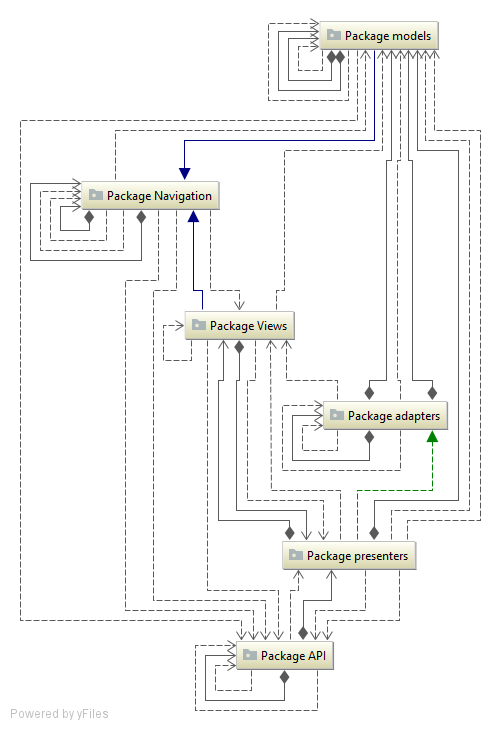
\includegraphics[width=12.5cm,height=6cm,keepaspectratio]{Obrazy/AM_DK_ALL}
			\caption{Schemat ogólny diagramu klas dla Aplikacji Mobilnej}
			\label{Schemat ogólny diagramu klas dla Aplikacji mobilnej}
		\end{figure}
	

		\begin{figure}[ht!]
		\centering
		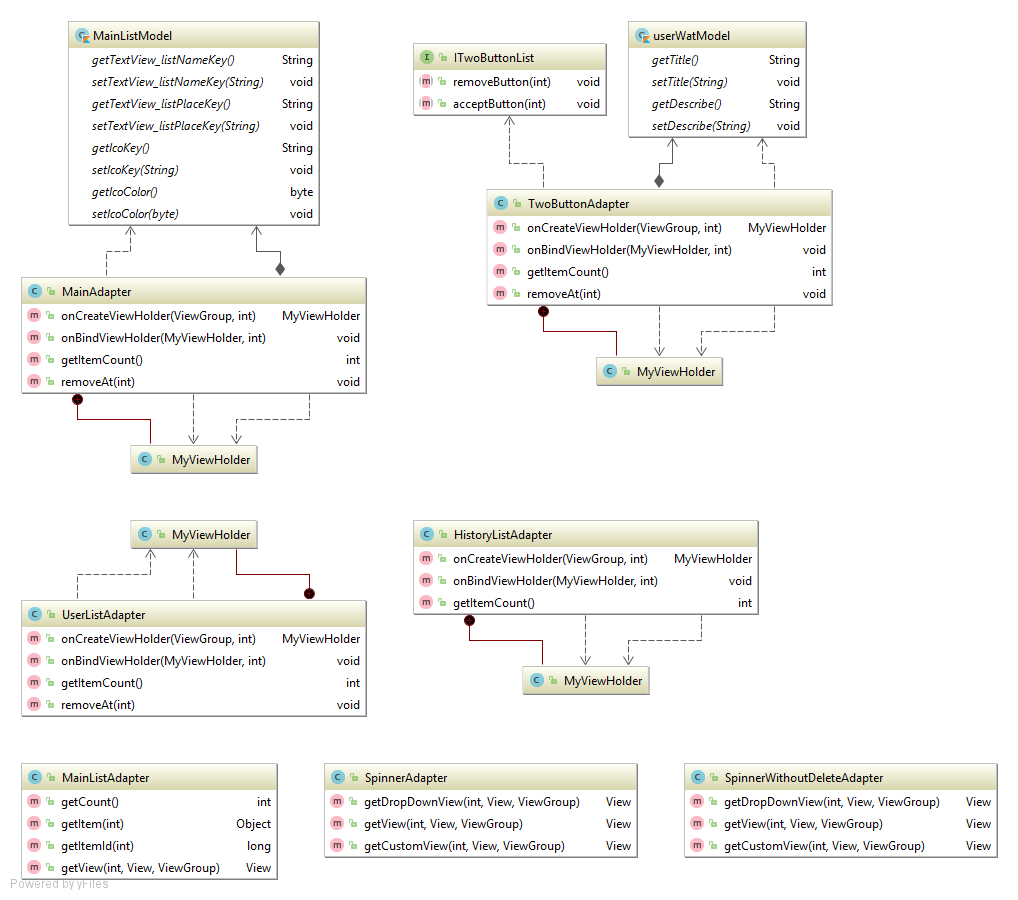
\includegraphics[width=12.5cm,height=10cm,keepaspectratio]{Obrazy/AM_DK_adapter}
		\caption{Diagram klas dla paczki adapters}
		\label{Diagram klas dla paczki adapters}
	\end{figure}


	
		\begin{figure}[ht!]
		\centering
		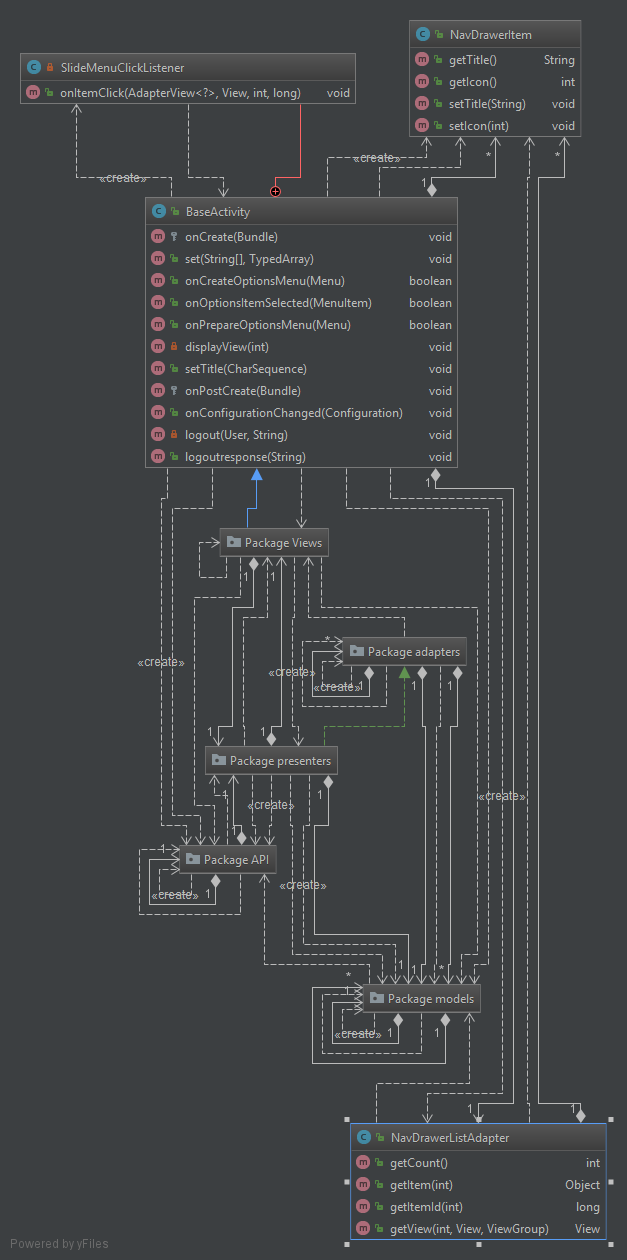
\includegraphics[width=12.5cm,height=10cm,keepaspectratio]{Obrazy/AM_DK_navigation}
		\caption{Diagram klas dla paczki navigations}
		\label{Diagram klas dla paczki navigations}
	\end{figure}

	
	
	
	
	\begin{figure}[ht!]
		\centering
		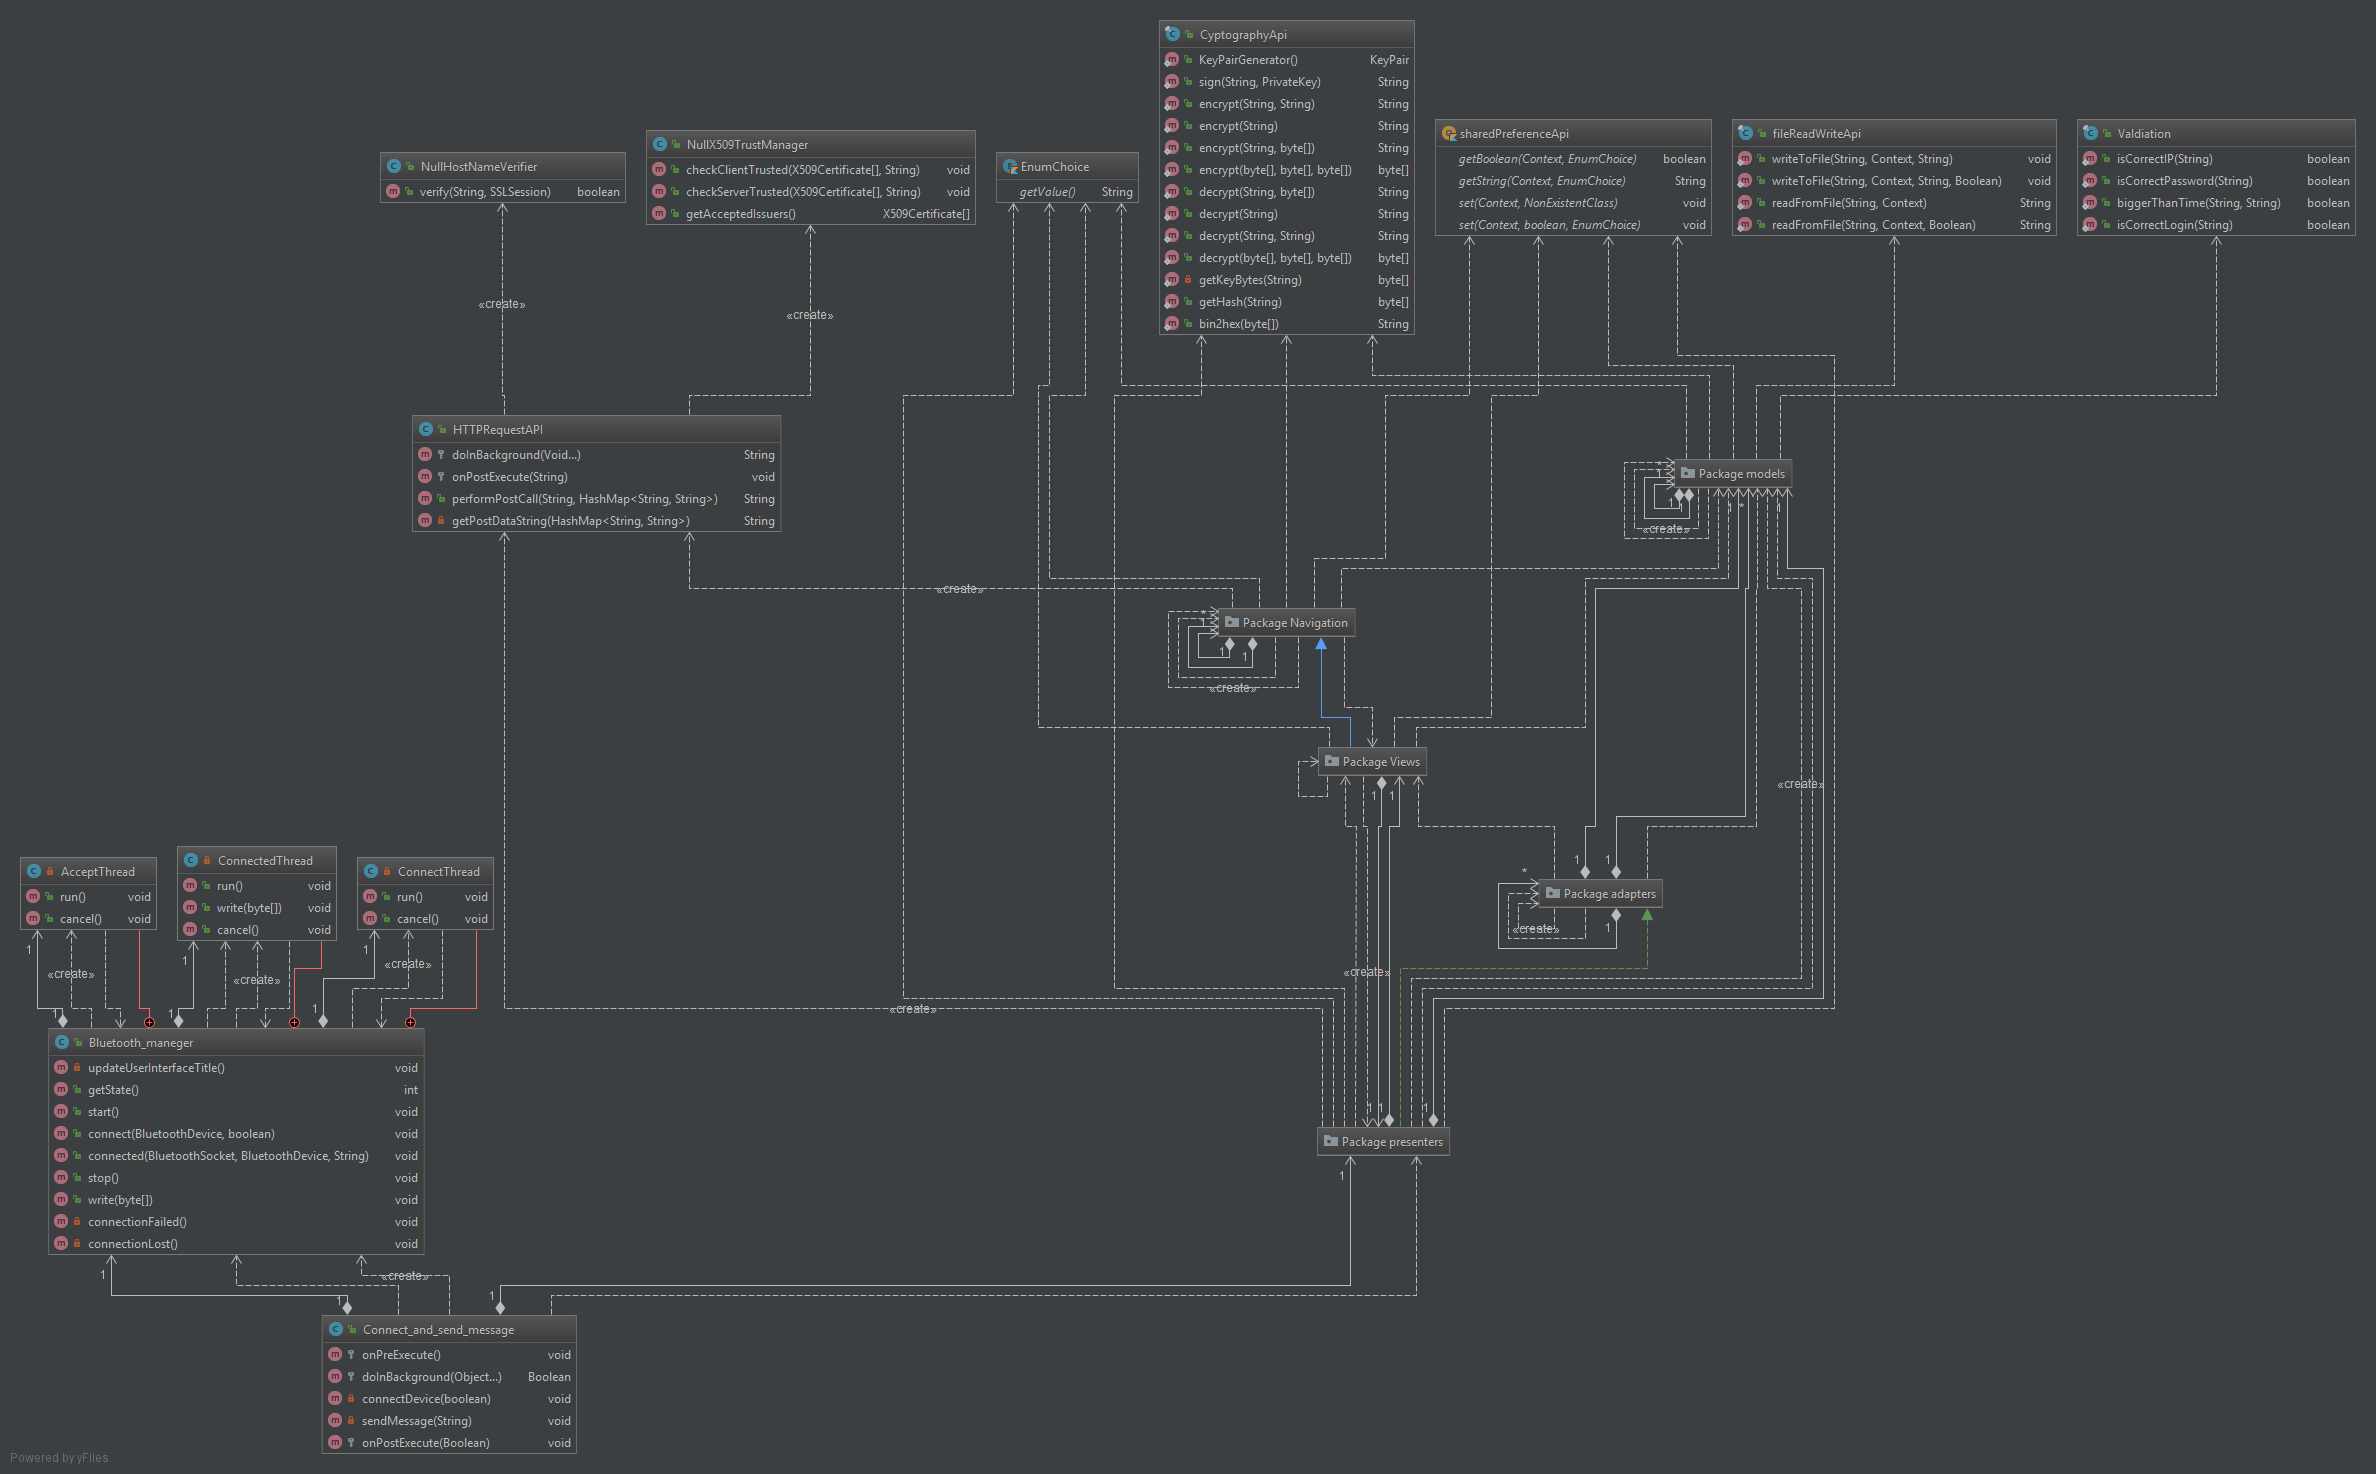
\includegraphics[width=12.5cm,height=16cm,keepaspectratio]{Obrazy/AM_DK_api}
		\caption{Diagram klas dla paczki api}
		\label{Diagram klas dla paczki api}
	\end{figure}

	

	\begin{figure}[ht!]
		\centering
		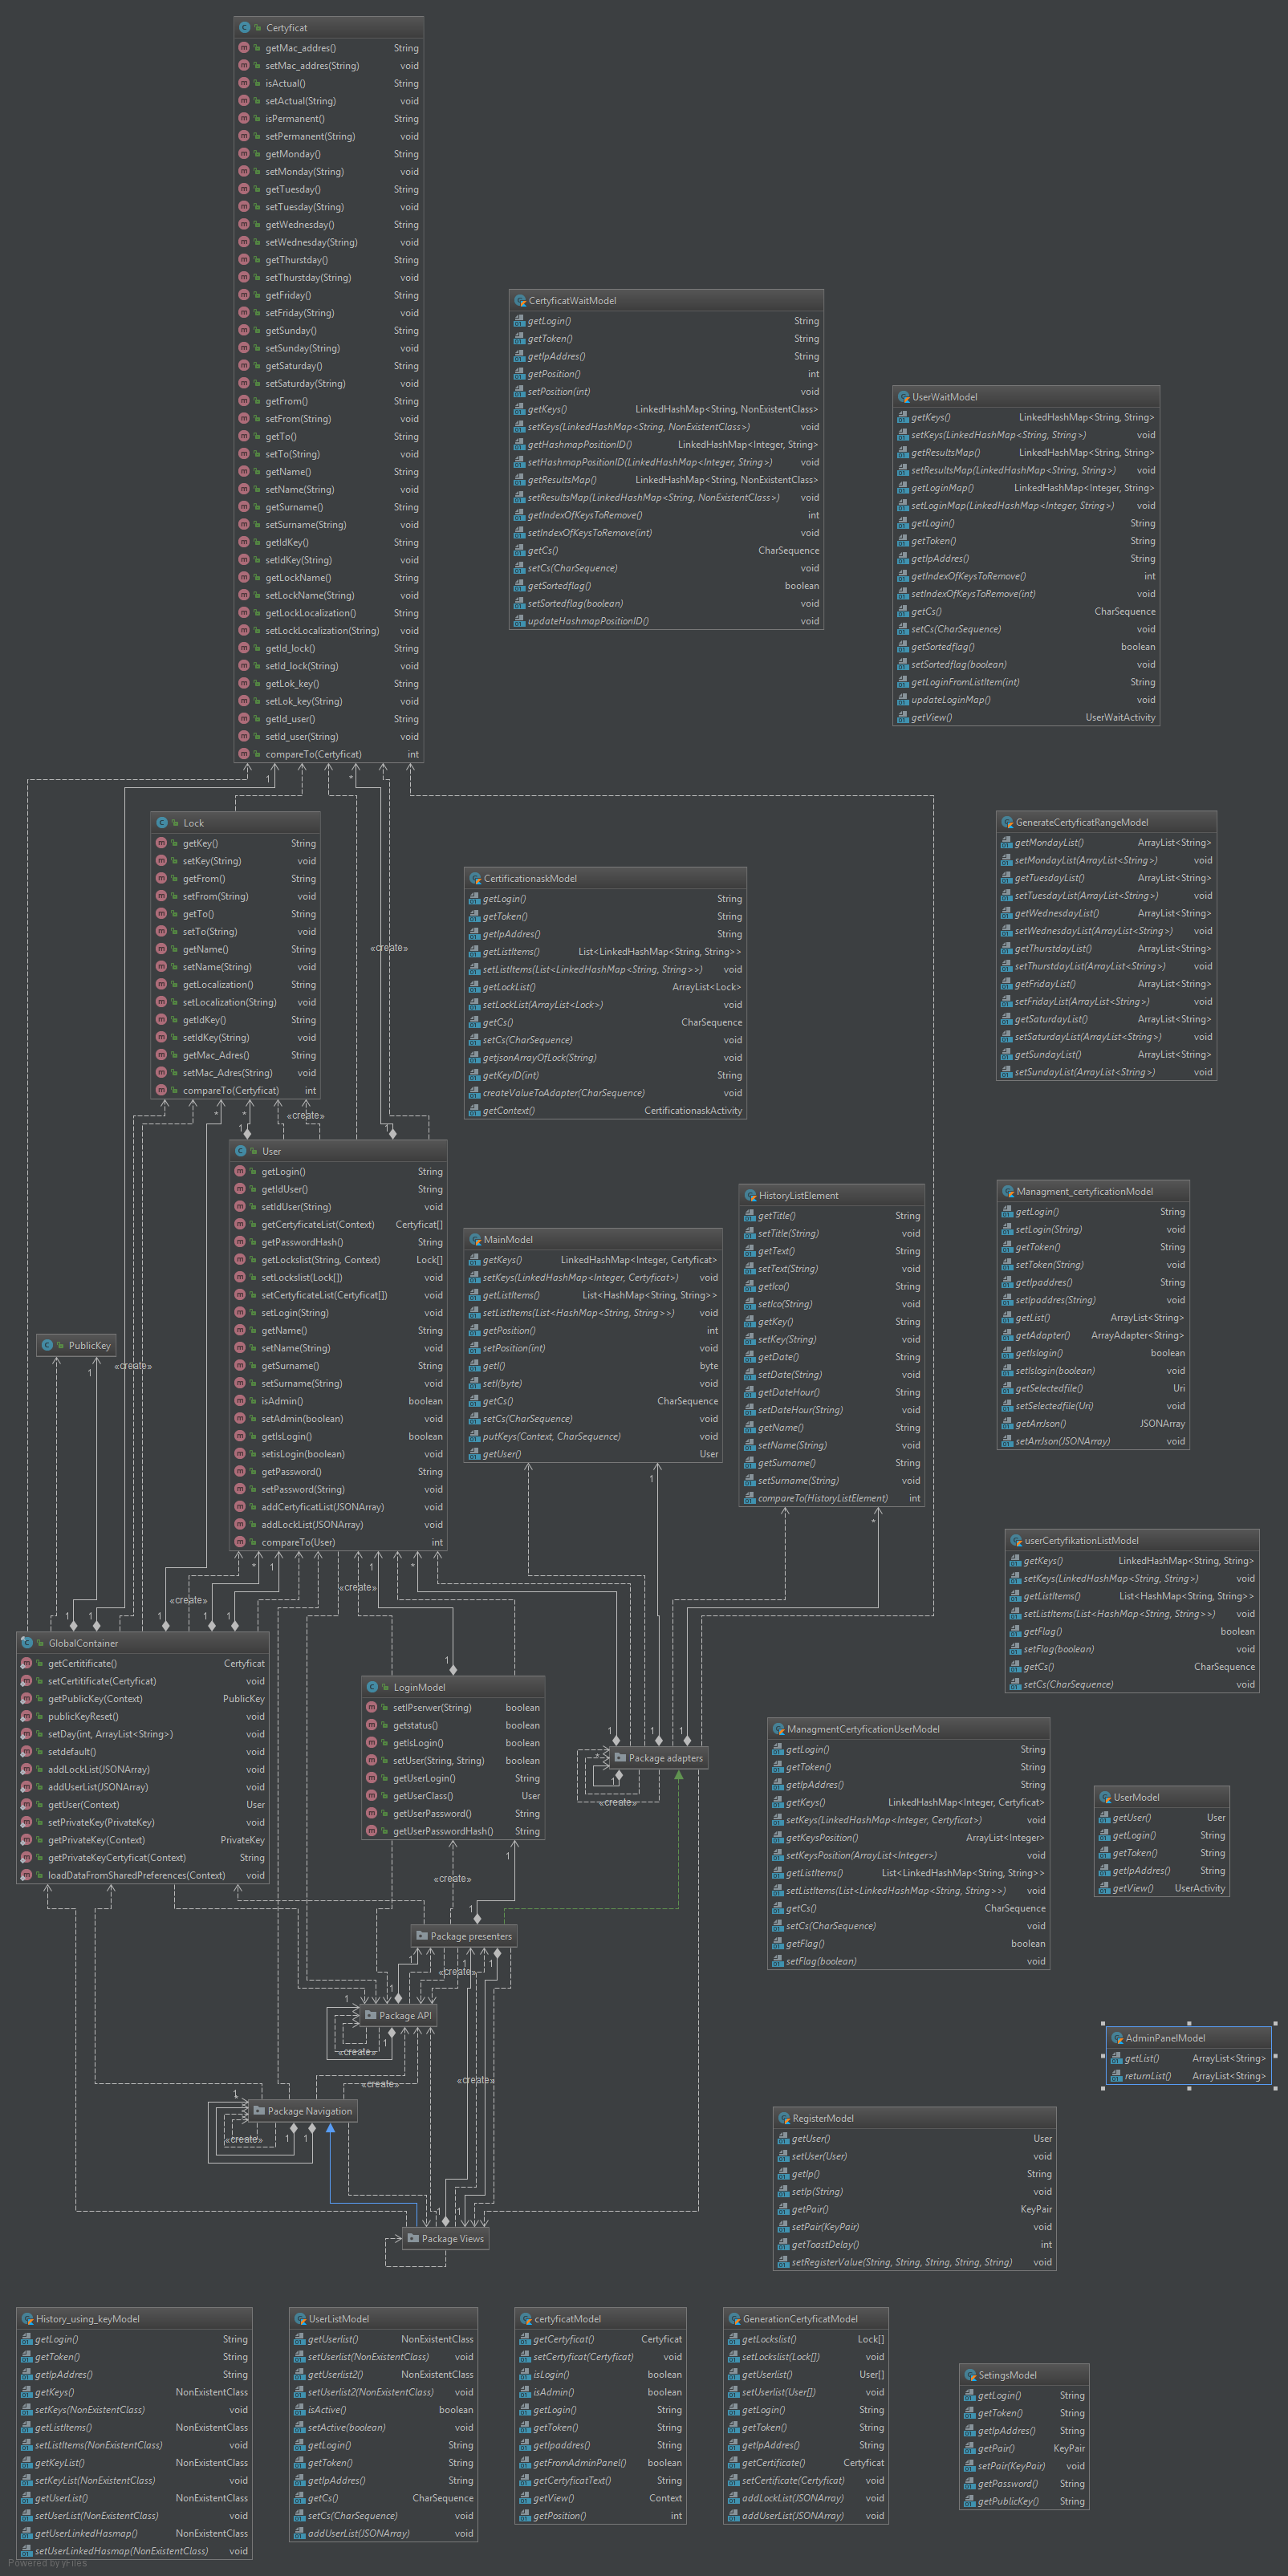
\includegraphics[width=12.5cm,height=16cm,keepaspectratio]{Obrazy/AM_DK_model}
		\caption{Diagram klas dla paczki models}
		\label{Diagram klas dla paczki models}
	\end{figure}

	
\begin{figure}[ht!]
	\centering
	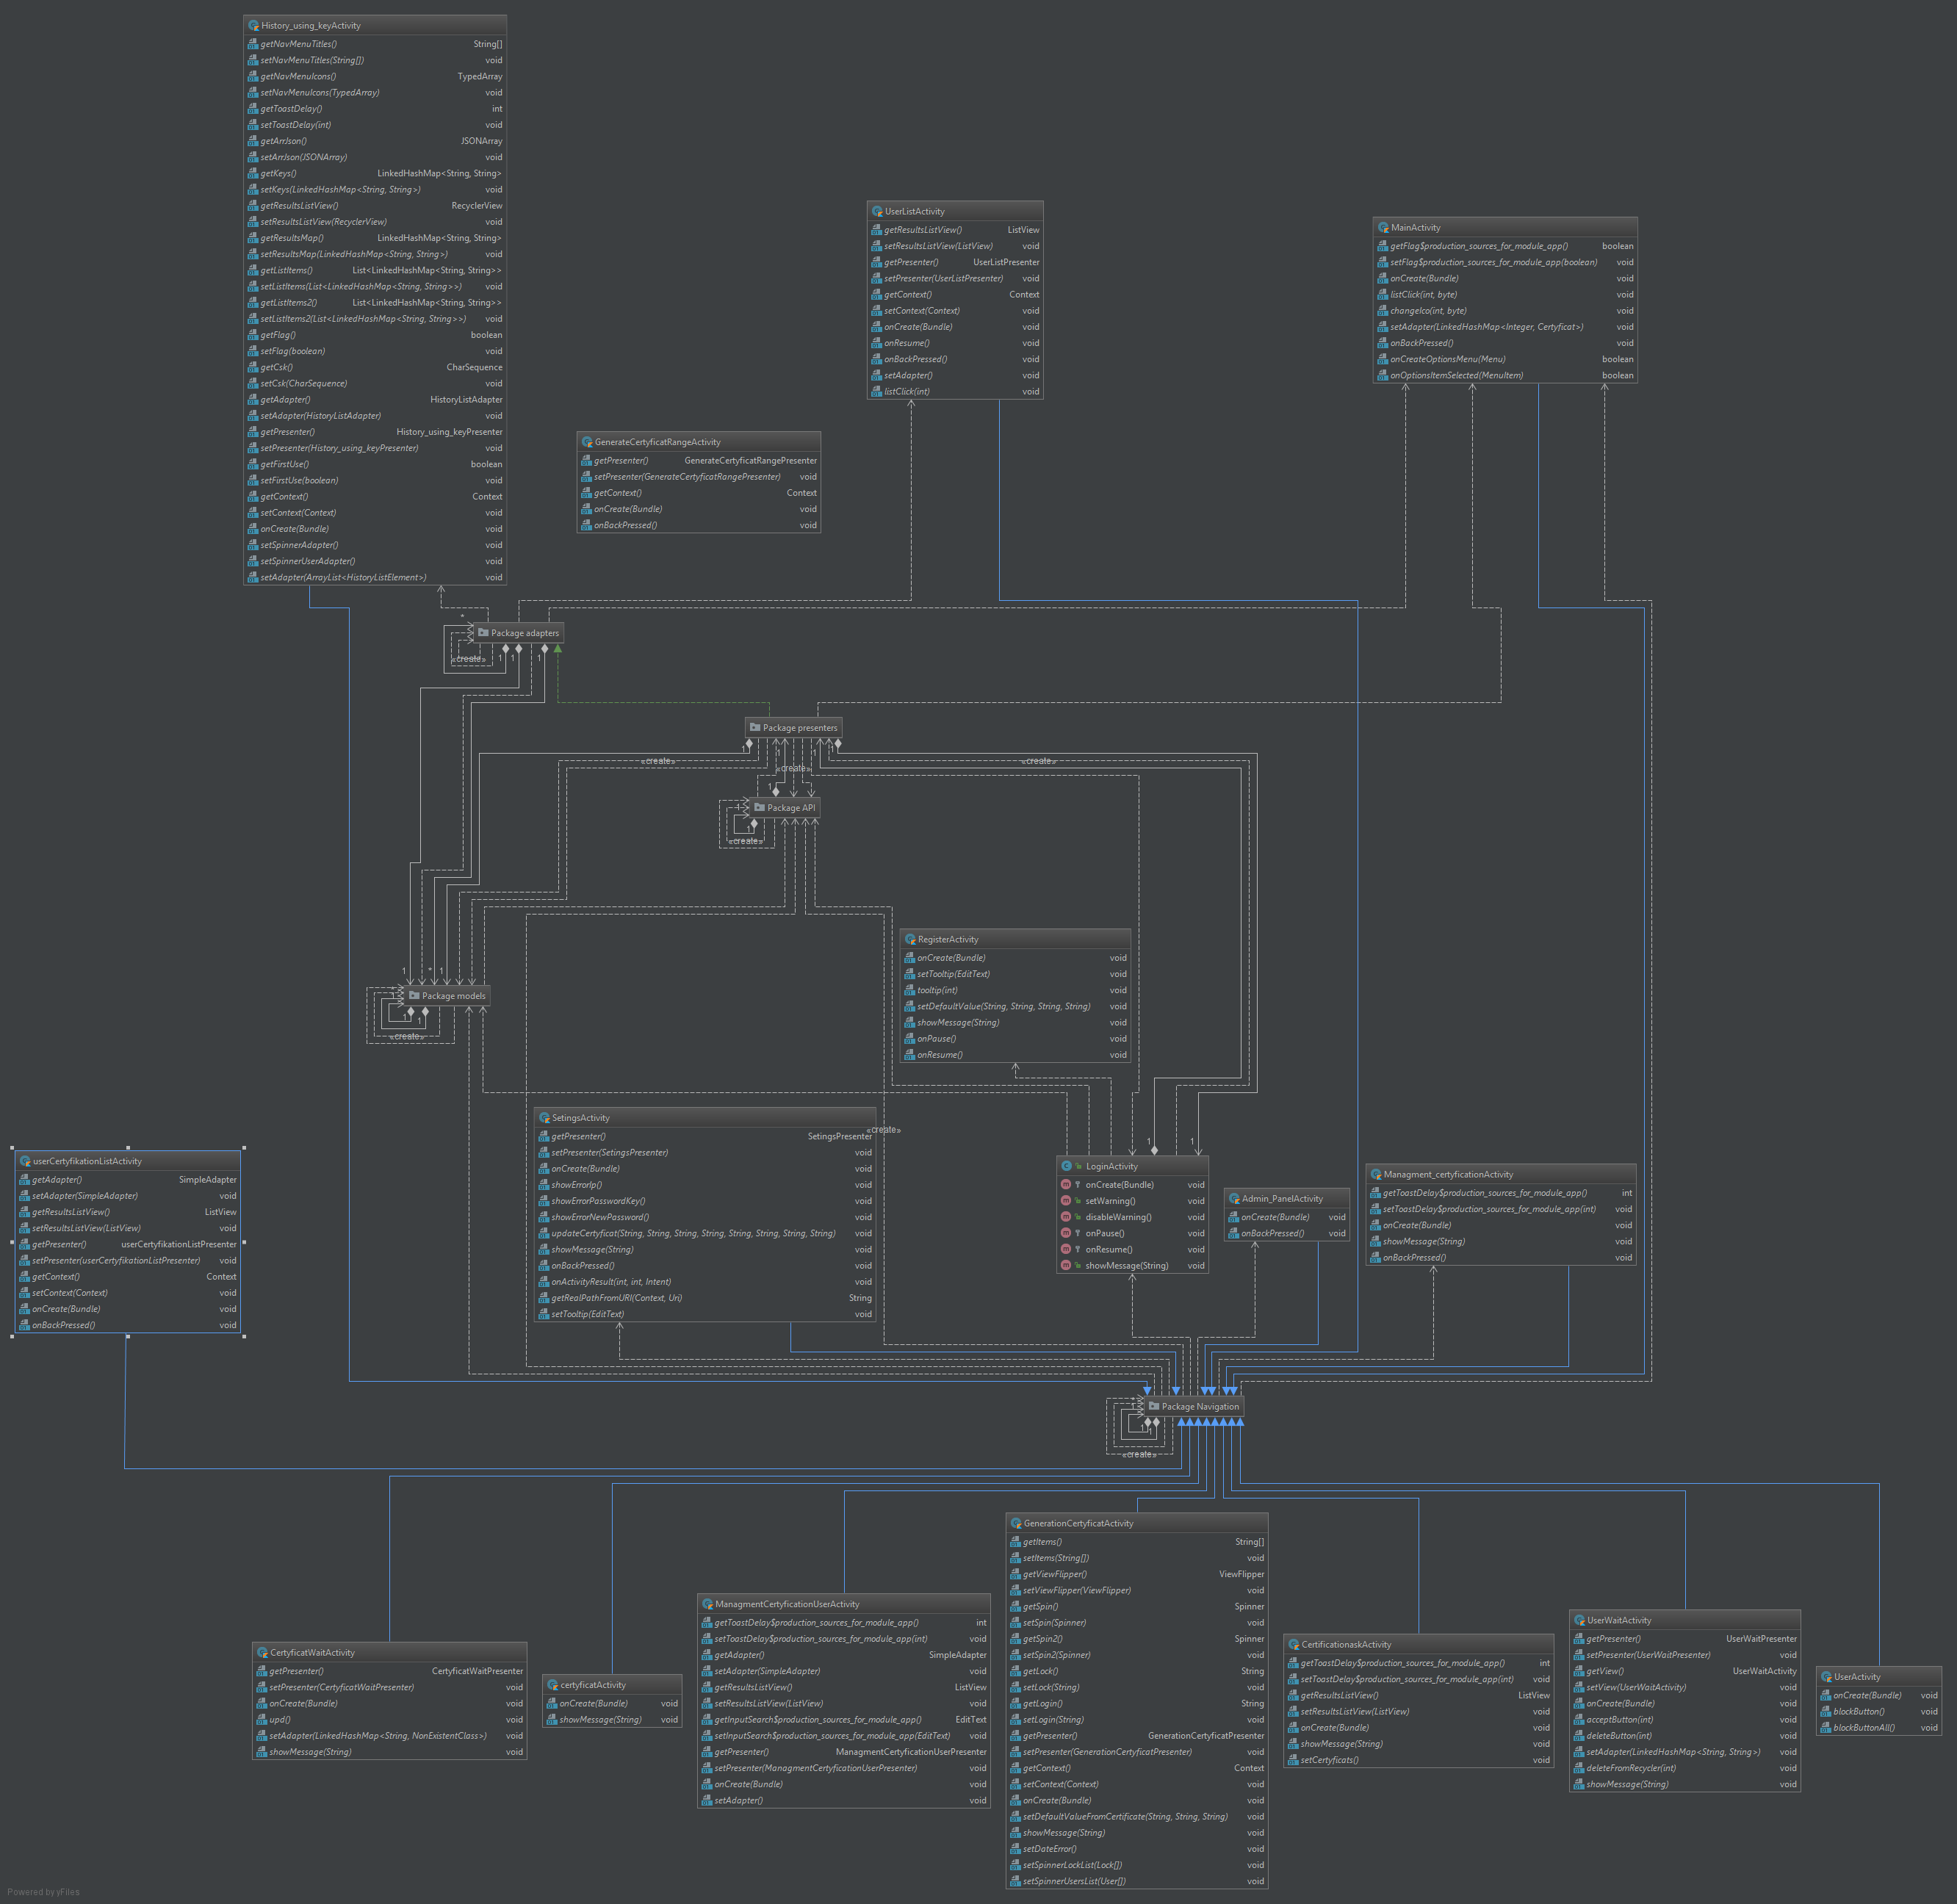
\includegraphics[width=12.5cm,height=12cm,keepaspectratio]{Obrazy/AM_DK_view}
	\caption{Diagram klas dla paczki views}
	\label{Diagram klas dla paczki views}
\end{figure}

		
			Ostatni diagram dotycząćy aplikacji mobilnej przedstawia rozwinięcie paczk Presenter wraz z połączeniami z innymi paczkami
		\begin{figure}[ht!]
			\centering
			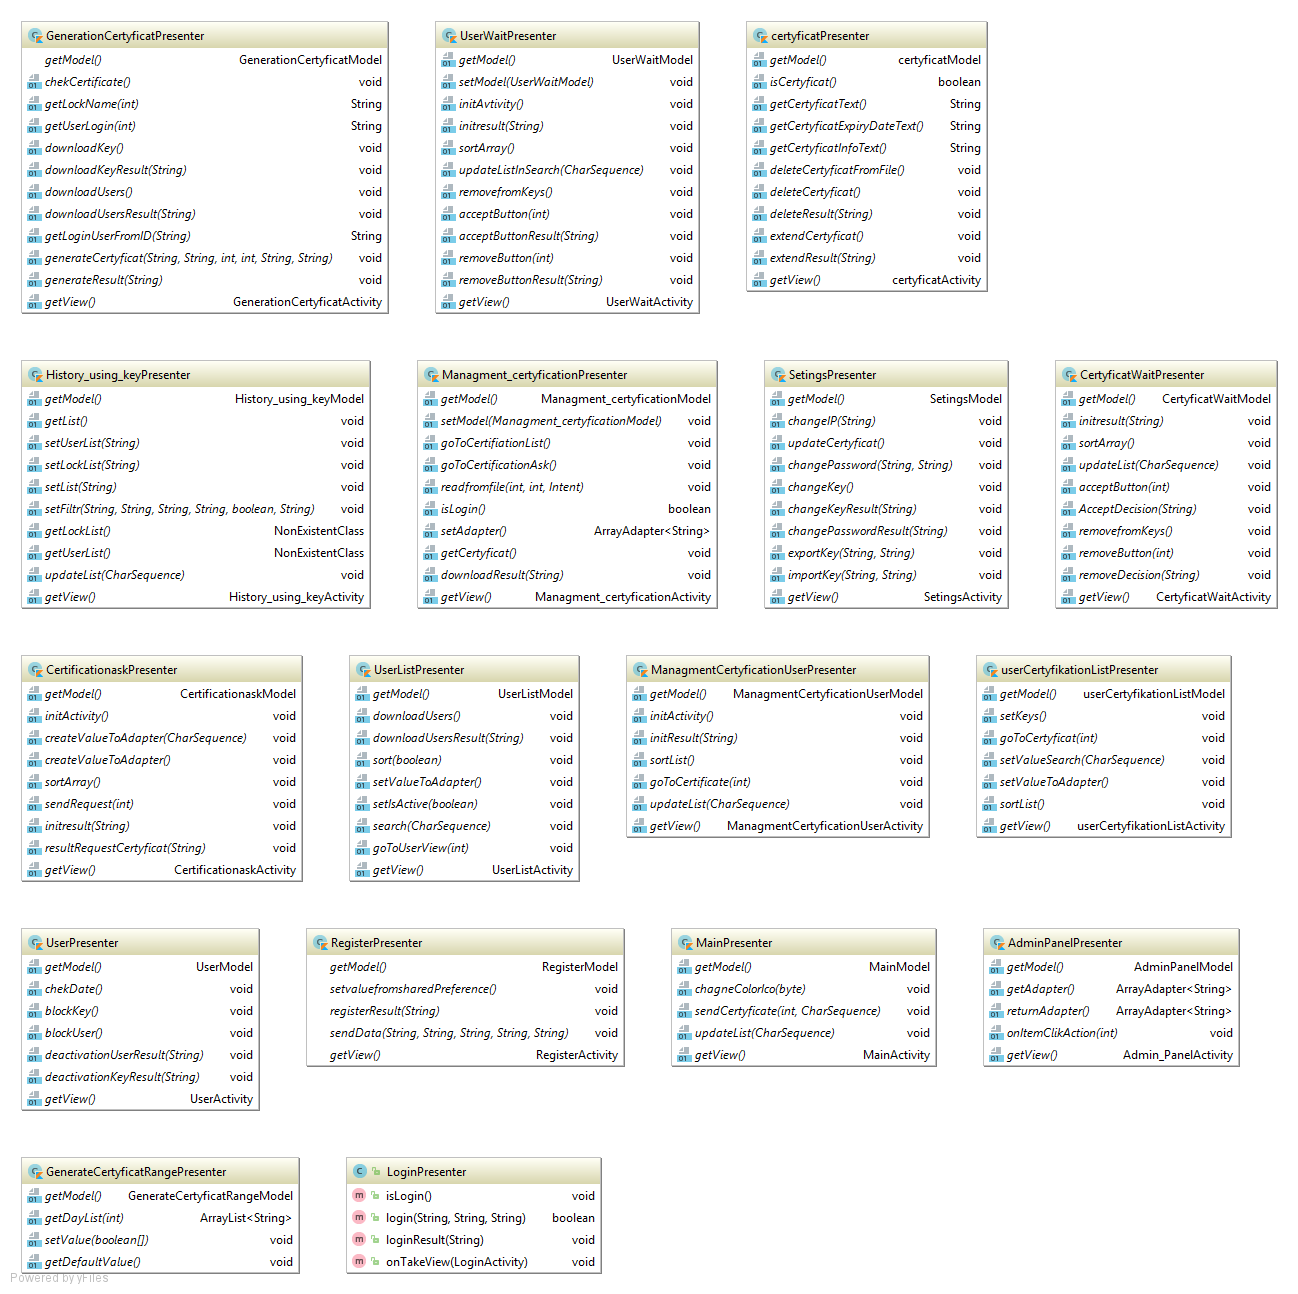
\includegraphics[width=12.5cm,height=14cm,keepaspectratio]{Obrazy/AM_DK_presenter}
			\caption{Diagram klas dla paczki presenters}
			\label{Diagram klas dla paczki presenters}
		\end{figure}
		
		\newpage
		\paragraph{Aplikacja serwera}
		\paragraph{Urządzenie sterujące}
		\paragraph{Moduł zliczania osób}

\newpage		
\subsection{Uproszczony schemat elektryczny systemu}

\newpage
\subsection{Komunikacja modułów systemu z aplikacją  serwera}

	\subsubsection{Komunikaty HTTPRequest pomiędzy aplikacją mobilną, \newline a serwerem}
	\subsubsection{Komunikaty HTTPRequest pomiędzy urządzeniem sterującym, a serwerem}
	
\newpage
\subsection{Protokoły komunikacji pomiędzy urządzeniem \newline sterującym i aplikacją mobilną}

\newpage
\subsection{Interfejs graficzny systemu}

	\subsubsection{Widoki aplikacji mobilnej}
		\section*{Panel logowania użytkownika}
	Widok umożliwia zalogowanie się użytkownika do systemu poprzez podanie loginu, hasła oraz adres IP serwera w odpowiednie pola, a następnie kliknięcie w przycisk “ZALOGUJ SIĘ”. Samo pole hasła jest maskowane. Jeśli nie posiada się konta, można je utworzyć poprzez przycisk “ZAREJESTRUJ SIĘ”. (Rysunek \ref{rys:panel_logowania_pionowo})
	
	\begin{figure}[ht!]
			\centering
			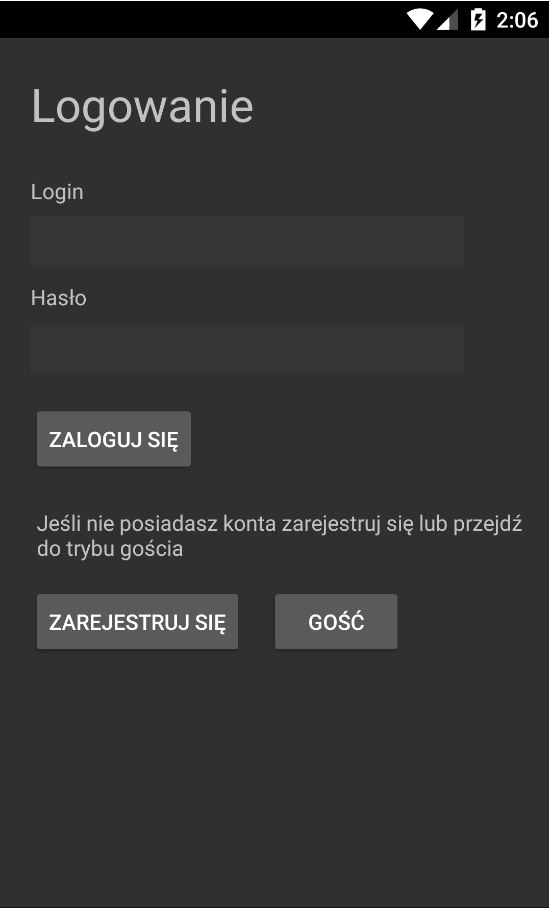
\includegraphics[width=12.5cm,height=8cm,keepaspectratio]
			{Obrazy/logowanie_uzytkownika_pionowo}
			\caption{Panel logowania użytkownika}
			\label{rys:panel_logowania_pionowo}
	\end{figure}

	
	\section*{Panel rejestracji użytkownika}
	Panel rejestracji służy do utworzenie nowego użytkownika poprzez podanie loginu, hasła, imienia i nazwiska użytkownika oraz adresu IP serwera do którego chcemy się zarejestrować. Pole z hasłem jest maskowane wraz z możliwośćią odkrywania hasłą przy pomocy ikonki oko Po upewnieniu się, że wszystkie dane są poprawne, aby zakończyć proces rejestracji, klikamy przycisk “ZAREJESTRUJ”. (Rysunek \ref{rys:panel_rejestracji_pionowo})
	
	\begin{figure}[ht!]
		\centering
		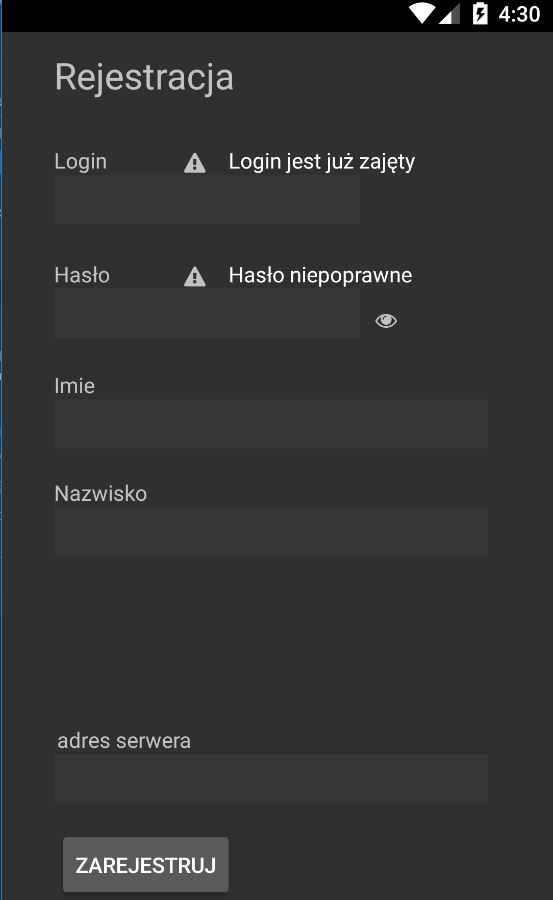
\includegraphics[width=12.5cm,height=8cm,keepaspectratio]
			{Obrazy/rejestracja_uzytkownika_pionowo}
			\caption{Panel logowania użytkownika }
			\label{rys:panel_rejestracji_pionowo}
		
	\end{figure}
	
	
	\section*{Panel listy zamków}
	Widok listy dostępnych zamków przedstawia listę nazw zamków do jakich dany użytkownik ma dostęp. Ułatwieniem jest możliwość sortowania wyników i wyszukiwanie po nazwach. Kliknięcie w nazwę zamka powoduje otwarcie zamka. Zmiana koloru ikon zamków sygnalizować ma status zamka.Opisy znaczeń poszcególnych koloróW oraz symboli opisane są w rozdziale symbolika oraz kolory. (Rysunek \ref{rys:panel_listy_dostepnych_zamkow_pionowo})
	
	\begin{figure}[ht!]
			\centering
		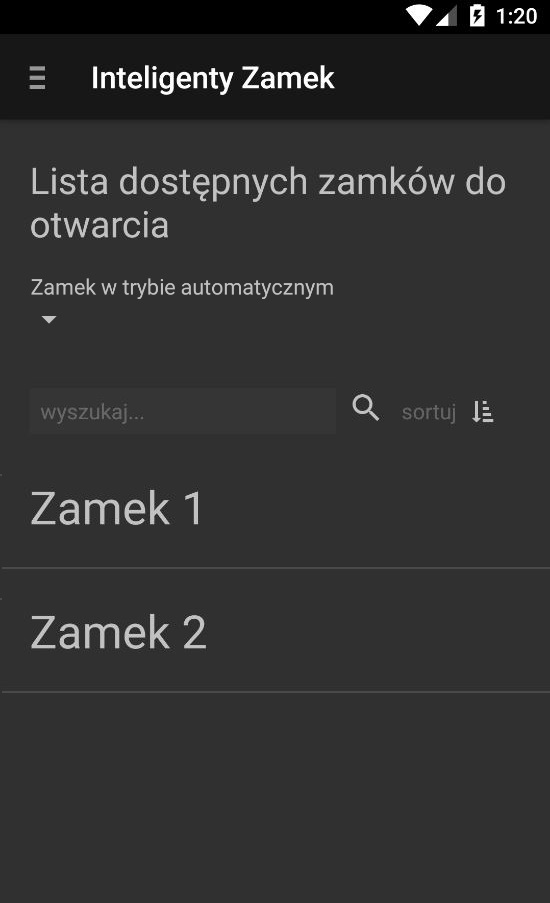
\includegraphics[width=12.5cm,height=8cm,keepaspectratio]
			{Obrazy/lista_dostepnych_zamkow_pionowo}
			\caption{Lista dostępnych zamków}
			\label{rys:panel_listy_dostepnych_zamkow_pionowo}
	
		
	\end{figure}
	
	
	\section*{Panel boczny}
	Panel boczny pozwala na szybkie przełączanie pomiędzy widokami. Chowany jest po lewej stronie ekranu. Umożliwia przechodzenie odpowiednio do listy zamków, zarządzania certyfikatami, panelu administracyjnego oraz ustawień. Ostatnia pozycja powoduje wylogowanie z aplikacji. Pnanel ten w zależnośći od uprawnień użytkownika możę posiadać lub nie pole z panelem administraotra (Rysunek \ref{rys:panel_boczny_pionowo} i \ref{rys:panel_boczny_pionowo2})
	
	\begin{figure}[ht!]
		\begin{minipage}{0.5\textwidth}
			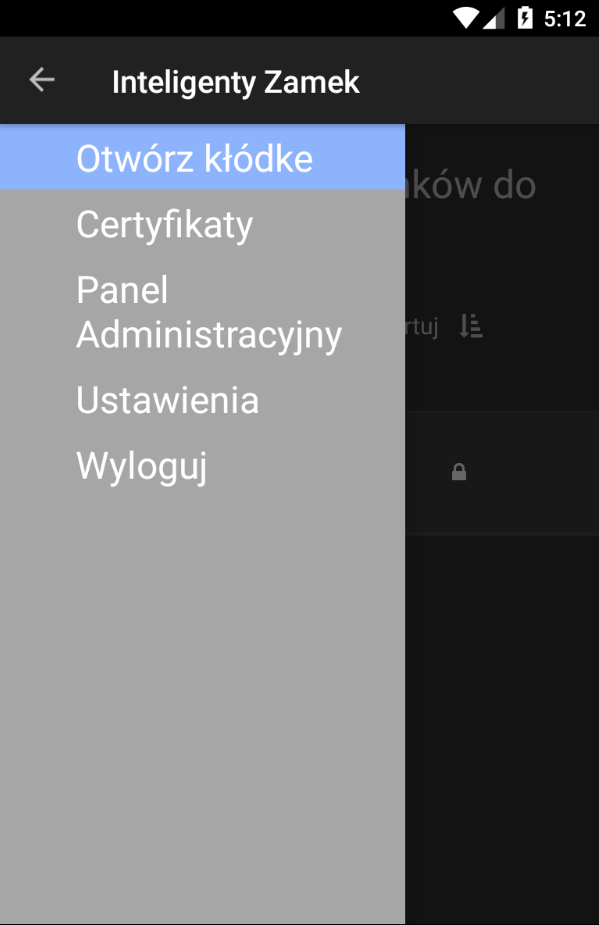
\includegraphics[width=\textwidth]
			{Obrazy/panel_boczny_pionowo}
			\caption{Panel boczny z uprawnieniami administratora}
			\label{rys:panel_boczny_pionowo}
		\end{minipage}
		\begin{minipage}{0.5\textwidth}
			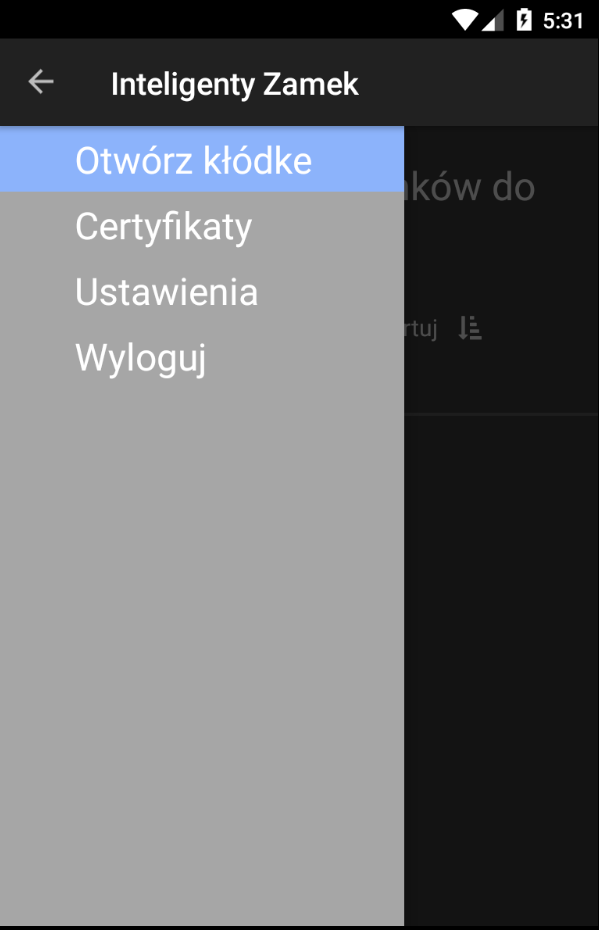
\includegraphics[width=\textwidth]{Obrazy/panel_boczny_pionowo2}
			\caption{Panel boczny bez uprawnieni administratora}
			\label{rys:panel_boczny_pionowo2}
		\end{minipage}	
	\end{figure}

	
	\section*{Panel zarządzania certyfikatami}
	Panel zarządzania certyfikatami umożliwia wybór funkcji dodania certyfikatu. Kolejne pozycje to lista posiadanych certyfikatów oraz wysłanie wniosku o utworzenie nowego certyfikatu  (Rysunek \ref{rys:panel_zarządzania_certyfikatami_pionowo})
	
	\begin{figure}[ht!]
		\centering
		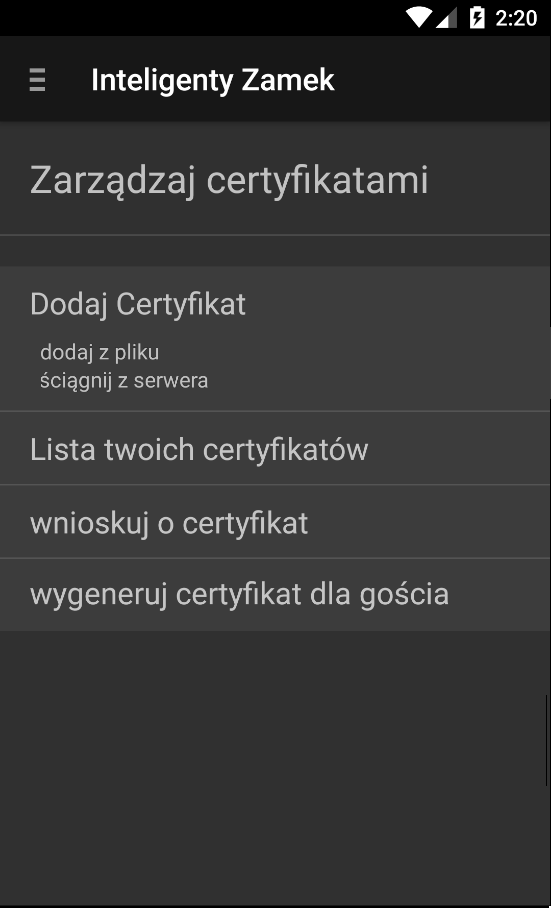
\includegraphics[width=12.5cm,height=8cm,keepaspectratio]
			{Obrazy/zarzadzaj_certyfikatami_pionowo}
			\caption{Panel zarządzania certyfikatami }
			\label{rys:panel_zarządzania_certyfikatami_pionowo}
		
	\end{figure}

	
	\section*{Panel listy certyfikatów}
	Panel listy certyfikatów, jest listą aktualnych certyfikatów należących do użytkownika. Kliknięcie w dany certyfikat przenosi do widoku szczegółowego związanego z operacjami na tym certyfikacie. (Rysunek \ref{rys:panel_listy_certyfikatów_pionowo} )
	
	\begin{figure}[ht!]
			\centering
	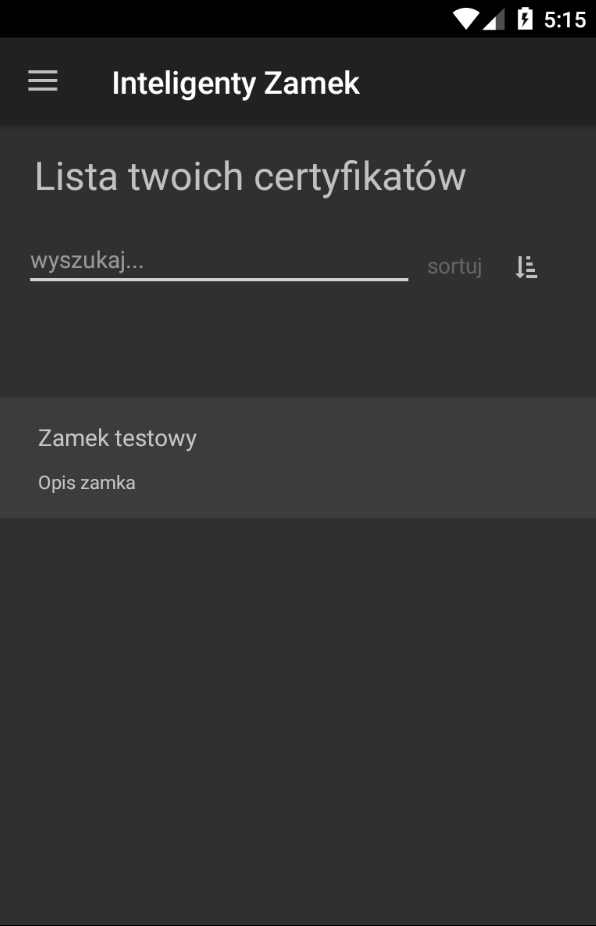
\includegraphics[width=12.5cm,height=8cm,keepaspectratio]
			{Obrazy/lista_certyfikatow_pionowo}
			\caption{Panel listy certyfikatów}
			\label{rys:panel_listy_certyfikatów_pionowo}
		
	\end{figure}

	
	\section*{Panel certyfikatu}
	Panel certyfikatu zawiera informacje o dacie wygaśnięcia, którego zamku dotyczy oraz w jakim czasie przyznaje dostęp. Na dole dostępne są dwa przyciski pozwalające usunąć certyfikat lub wysłać prośbę o przedłużenie ważności. W zależnośći od tego czy uzytkownik ma uprawnienia administratora przycisk przedłuż certyfikat albo wyśle zgłoszenie do serwera (dla użytkownika bez uprawnieni administratora) albo przeniesie do panelu generowania certyfikatu (dla użytkownika o uprawnieniach administratora) (Rysunek \ref{rys:panel_certyfikatu_pionowo})
	
	\begin{figure}[ht!]
		\centering
		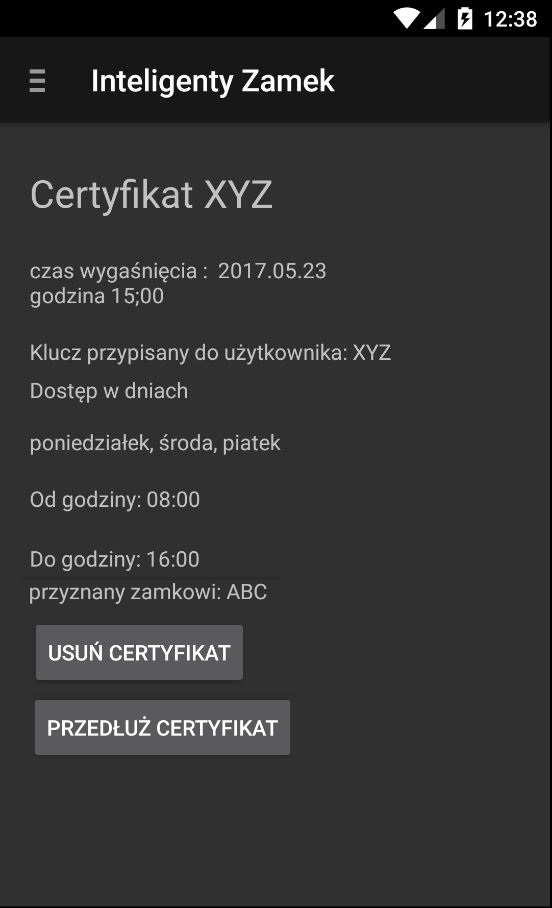
\includegraphics[width=12.5cm,height=8cm,keepaspectratio]
			{Obrazy/certyfikat_pionowo}
			\caption{Panel certyfikatu }
			\label{rys:panel_certyfikatu_pionowo}
		
	\end{figure}
	
	\section*{Panel wnioskowania o certyfikat}
	Panel wnioskowania o certyfikat polega na wybraniu z listy wszystkich zamków, konkretnego do którego chcemy uzyskać dostęp i wysłać wniosek o przydzielenie dostępu. (Rysunek \ref{rys:panel_wnioskowania_o_certyfikat_pionowo})
	
	\begin{figure}[ht!]
		\centering
		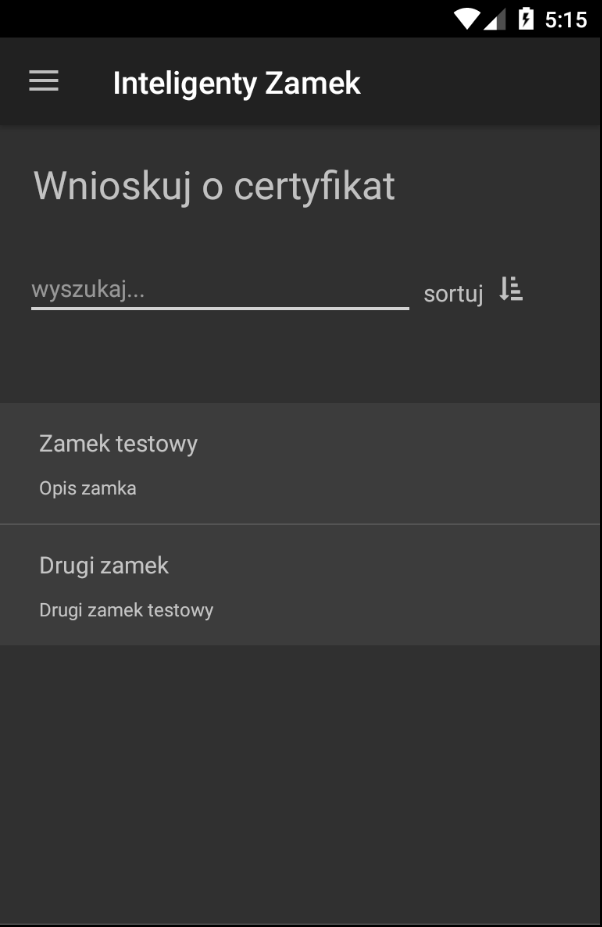
\includegraphics[width=12.5cm,height=8cm,keepaspectratio]
			{Obrazy/wnioskuj_o_certyfikat_pionowo}
			\caption{Panel wnioskowania o certyfikat }
			\label{rys:panel_wnioskowania_o_certyfikat_pionowo}
	
	\end{figure}
	
	
	\section*{Panel administratora}
	W panelu administratora znajdują się 6 przycisków do administrowania systemem zamków:
	\begin{itemize*}
		\item ,,Historia użycia zamków''
		\item ,,Generowanie nowego certyfikatu'',
		\item ,,Zarządzanie certyfikatami użytkowników'',
		\item ,,Lista oczekujących użytkowników do zarejestrowania'',
		\item ,,Lista oczekujących certyfikatów do zaakceptowania'',
		\item ,,Zarządzanie kontami użytkowników''.
	\end{itemize*}
	
	Po kliknięciu każdego przycisku przechodzi się do nowego odpowiadającego widoku. (Rysunek \ref{rys:panel_administracyjny_pionowo})
	
	\begin{figure}[ht!]
			\centering
	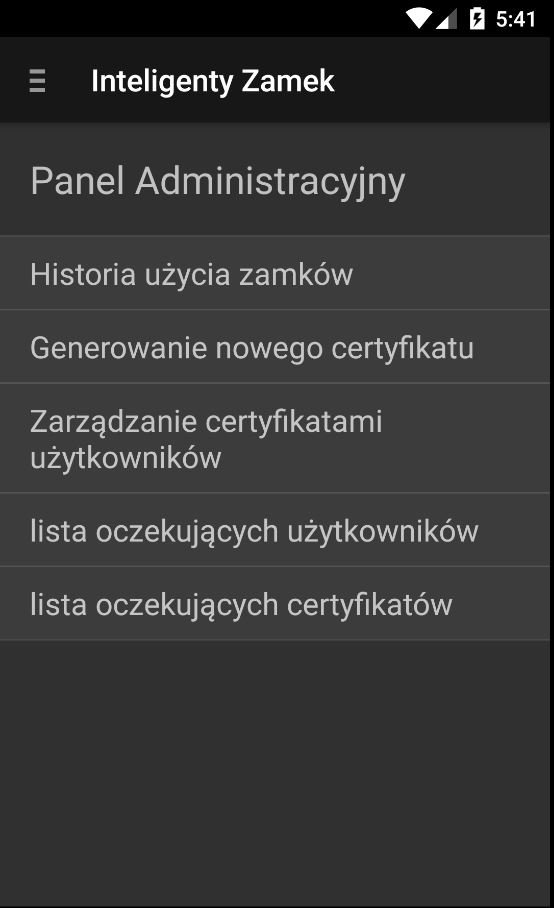
\includegraphics[width=12.5cm,height=8cm,keepaspectratio]
			{Obrazy/panel_administracyjny_pionowo}
			\caption{Panel administratora}
			\label{rys:panel_administracyjny_pionowo}
	
	\end{figure}

	
	\section*{Panel historii użycia zamków}
	Panel historii użycia zamków składa się z rozwijanej listy filtorwania histori w której są elementy takie jak lista dostępnych zamkóW, lista dostępnych uzytkowników, data podług której następuje filtracja oraz chekbox do zaznaczania czy tylko były nieautoryzowane próby. By uzyskać daną filtrację należy nacisnać przycisk filtruj. Oprócz panelu do filtrowania znajduje się również sama historia gdzie wyświetlane jestrodzaj próby otwarcia, data oraz przez kogo była ta próba podjęta. (Rysunek \ref{rys:panel_historii_uzycia_zamka_pionowo} i \ref{rys:panel_historii_uzycia_zamka_pionowo2})
	
	\begin{figure}[ht!]
		\begin{minipage}{0.5\textwidth}
			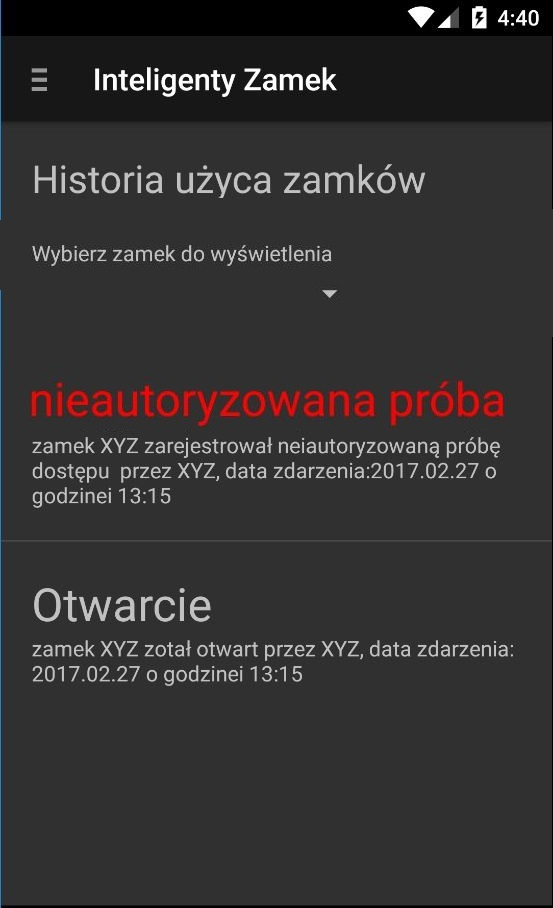
\includegraphics[width=\textwidth]{Obrazy/historia_zamkow_pionowo}
			\caption{Panel historii użycia zamków (filtr)}
			\label{rys:panel_historii_uzycia_zamka_pionowo}
		\end{minipage}
		\begin{minipage}{0.5\textwidth}
			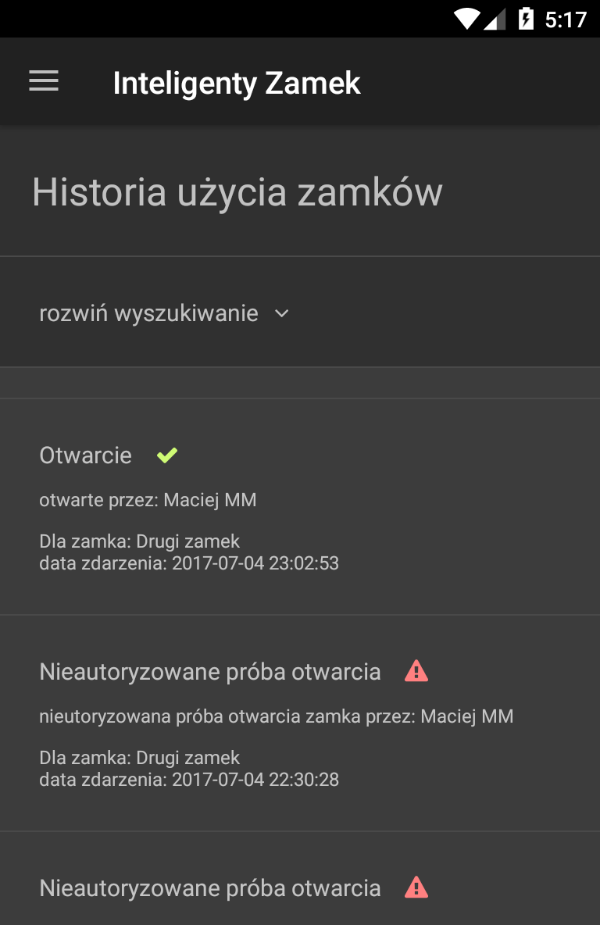
\includegraphics[width=\textwidth]{Obrazy/historia_zamkow_pionowo2}
			\caption{Panel historii użycia zamków (historia)}
			\label{rys:panel_historii_uzycia_zamka_pionowo2}	
		\end{minipage}
	\end{figure}
	\newpage
	
	\section*{Panel generowania nowego certyfikatu (administrator)}
	Panel generowanie nowego certyfikatu (administrator) służy do tworzenia nowych certyfikatów przez administratora. W pierwszych polach podaje się imię i nazwisko kogo dotyczy certyfikat.Następnie wybierane jest użytkownik (login) oraz zamek z rozwijanej listy. W dalszej części wybierane jest zakres dat w których certyfikat ma być ważny. Potem widać przycisk o nazwie "zakres obowiązywania certyfikatów" który przekierowywuje do widoku odpowiedzialnego za to w jakich godzinach dla danych dni tygodni certyfikat udziela dostępu. (Rysunek \ref{rys:panel_generowanie_nowego_klucza_gosc_admin_pioniowo}, \ref{rys:panel_generowanie_nowego_klucza_admin_pionowo2} i 
	\ref{rys:panel_wyboru_zakresu_certyfikatu})
	
	\begin{figure}[ht!]
		\vspace{-0.5cm}
		\begin{minipage}{0.5\textwidth}
			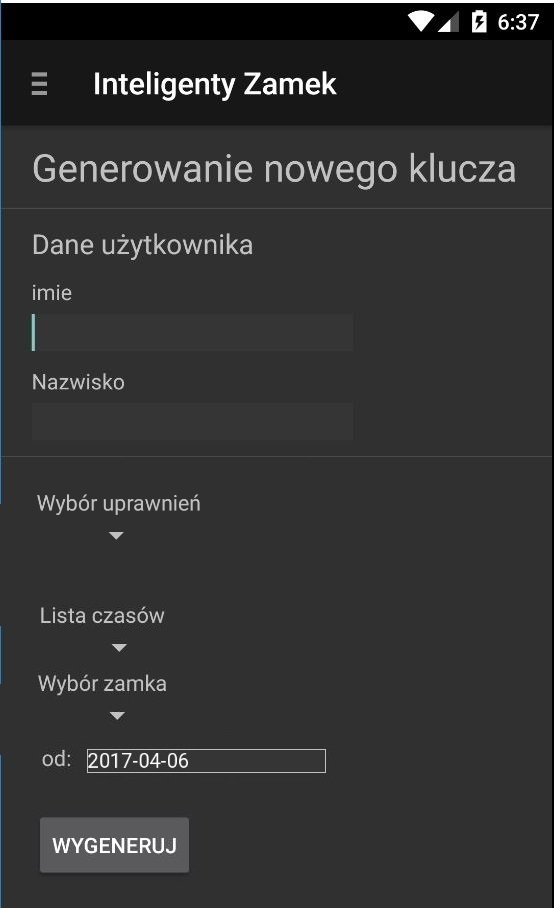
\includegraphics[width=\textwidth]{Obrazy/generowanie_nowego_klucza_gosc_admin_pioniowo}
			\caption{Panel generowania nowego klucza cz. 1 }
			\label{rys:panel_generowanie_nowego_klucza_gosc_admin_pioniowo}
		\end{minipage}
		\hspace{0.5cm}
		\begin{minipage}{0.5\textwidth}
			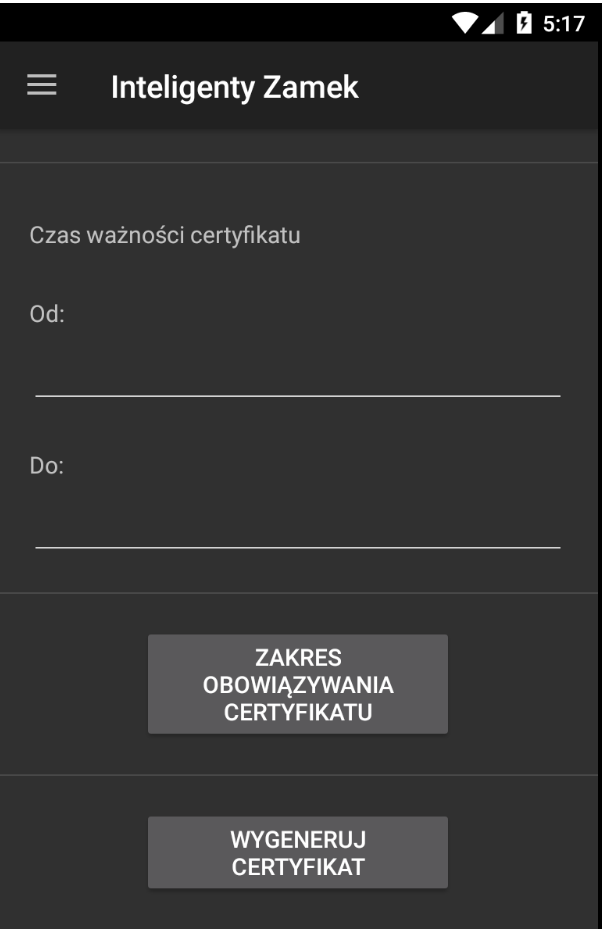
\includegraphics[width=\textwidth]{Obrazy/generowanie_nowego_klucza_admin_pionowo2}
			\caption{Panel generowania nowego klucza cz. 2}
			\label{rys:panel_generowanie_nowego_klucza_admin_pionowo2}	
		\end{minipage}
	\end{figure}
	\vspace{-0.5cm}
	\begin{figure}[ht!]
		\center
			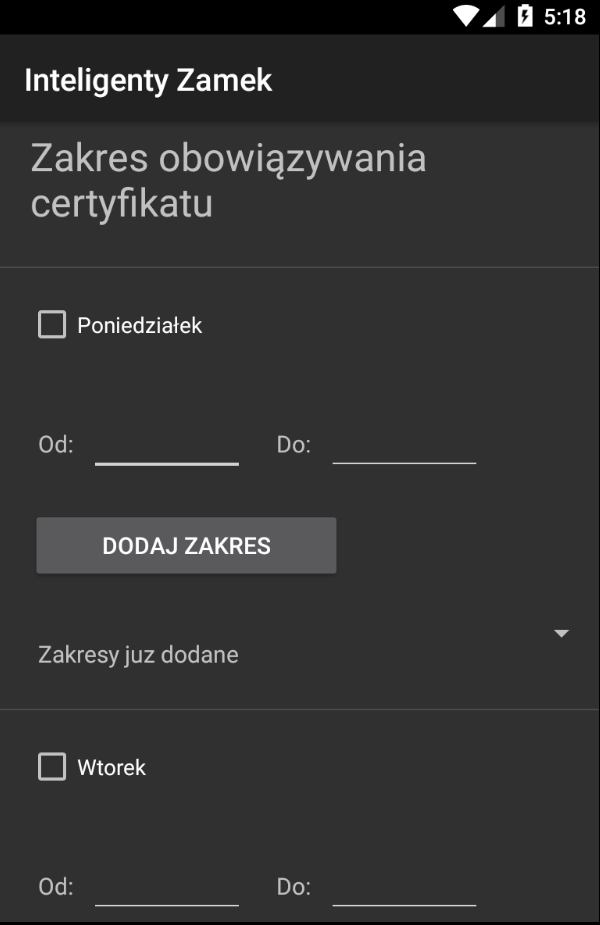
\includegraphics[width=4.5cm]{Obrazy/generowanie_nowego_klucza_uzytkownik_zalogowany_admin_pioniowo}
			\caption{Panel generowania nowego klucza dla użytkownika }
			\label{rys:panel_generowanie_nowego_klucza_uzytkownik_zalogowany_admin_pioniowo}
	\end{figure}

	
	\section*{Panel zarządzania certyfikatami~(administrator)}
	Panel zarządzania certyfikatami użytkowników (administrator) jest widokiem tylko wszystkich aktywnych certyfikatów w systemie. Administrator klikając na pozycję przechodzi do panelu certyfikatu opisanego wyżej. Tam może usunąć dostęp lub go przedłużyć. Ułatwieniem jest możliwość wyboru typu sortowania. (Rysunek \ref{rys:panel_lista_certyfikatow_administrator_pionowo})
	
	\begin{figure}[ht!]
		\centering
	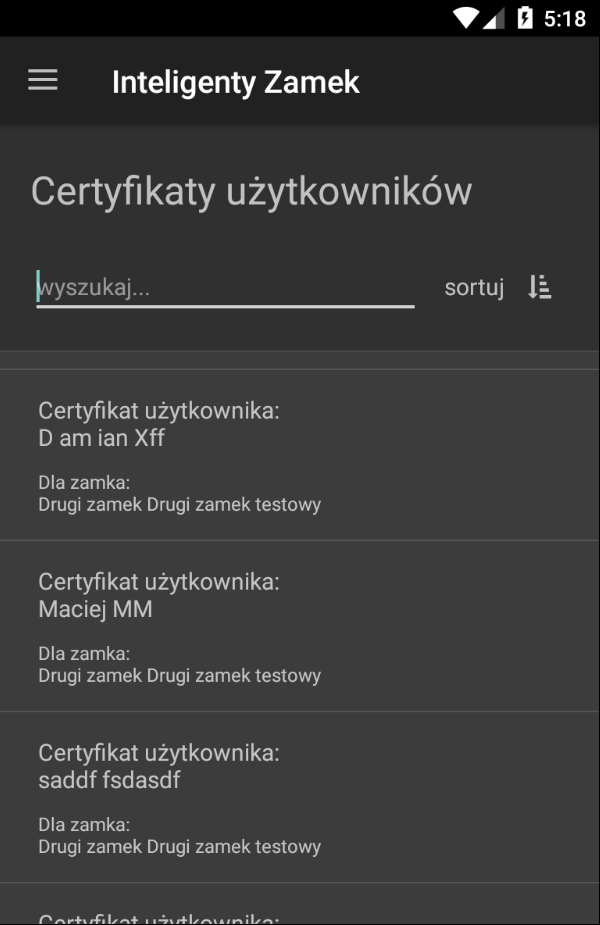
\includegraphics[width=12.5cm,height=8cm,keepaspectratio]
			{Obrazy/lista_certyfikatow_administrator_pionowo}
			\caption{Panel zarządzania certyfikatami (administrator) }
			\label{rys:panel_lista_certyfikatow_administrator_pionowo}
	
	\end{figure}

	
	\section*{Panel~listy~oczekujących~użytkowników~do~rejestracji}
	Panel listy oczekujących użytkowników jest listą wszystkich gości, którzy ubiegają się o zarejestrowanie. PO kliknięciu w odpowiednią pozycję pojawiają się dwie opcję: “AKCEPTUJ” lub “ODRZUĆ”.  (Rysunek \ref{rys:panel_lista_oczekujacych_uzytkownikow_pionowo} )
	
	\begin{figure}[ht!]
		\centering
	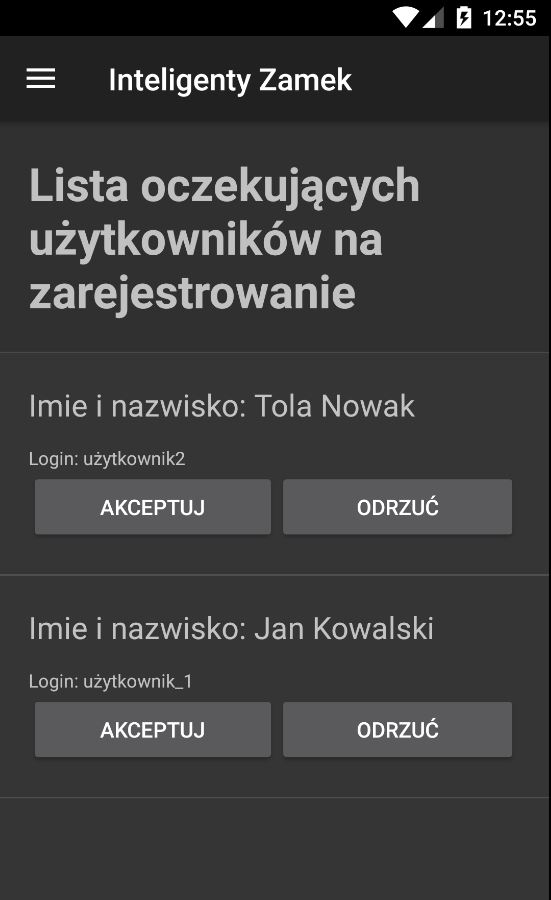
\includegraphics[width=12.5cm,height=8cm,keepaspectratio]
			{Obrazy/lista_oczekujacych_uzytkownikow_pionowo}
			\caption{Panel listy oczekujących użytkowników }
			\label{rys:panel_lista_oczekujacych_uzytkownikow_pionowo}
	
	\end{figure}

	
	\section*{Panel~listy~oczekujących~certyfikatów do~wygenerowania}
	Panel listy oczekujących certyfikatów jest listą wszystkich certyfikatów, które ubiegają się o akceptację administratora. Po kliknięciu w odpowiednią pozycję pojawiają się dwie opcję: “AKCEPTUJ” lub “ODRZUĆ”.  (Rysunek \ref{rys:panel_lista_oczekujacych_certyfikatow_pionowo} )
	
	\begin{figure}[ht!]
			\centering
			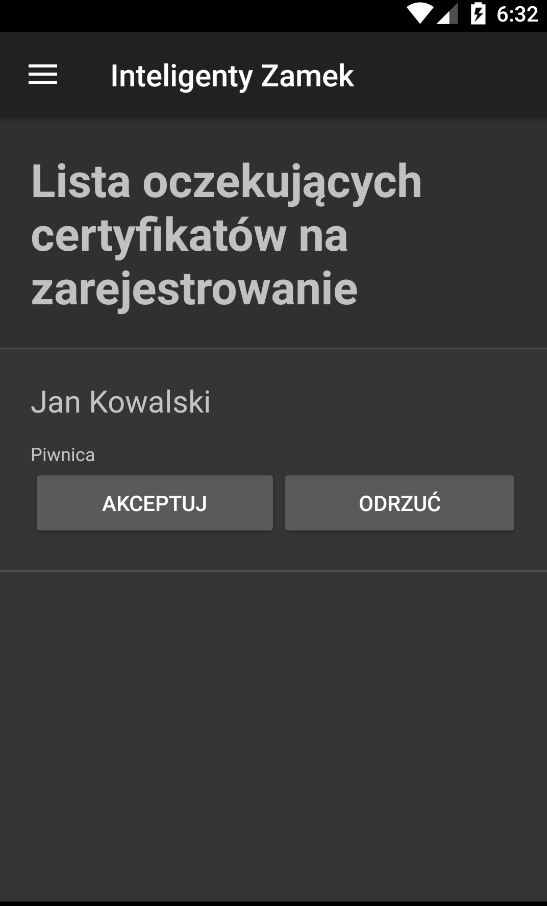
\includegraphics[width=12.5cm,height=8cm,keepaspectratio]
			{Obrazy/lista_oczekujacych_certyfikatow_pionowo}
			\caption{Panel listy oczekujących certyfikatów }
			\label{rys:panel_lista_oczekujacych_certyfikatow_pionowo}
		
	\end{figure}
	
	\section*{Panel zarządzania kontami użytkowników}
	Panel ten służy do zarządzania kontami użytkowników. Wyświetla on listę użytkownikóW systemu wraz z zonaczeniami czy jest on aktyny bądż zablokowany oraz czy ma ważny klucz szyfrujący (Rysunek \ref{rys:panel_Zarządzania_Kontami})
	
	\begin{figure}[ht!]
			\centering
			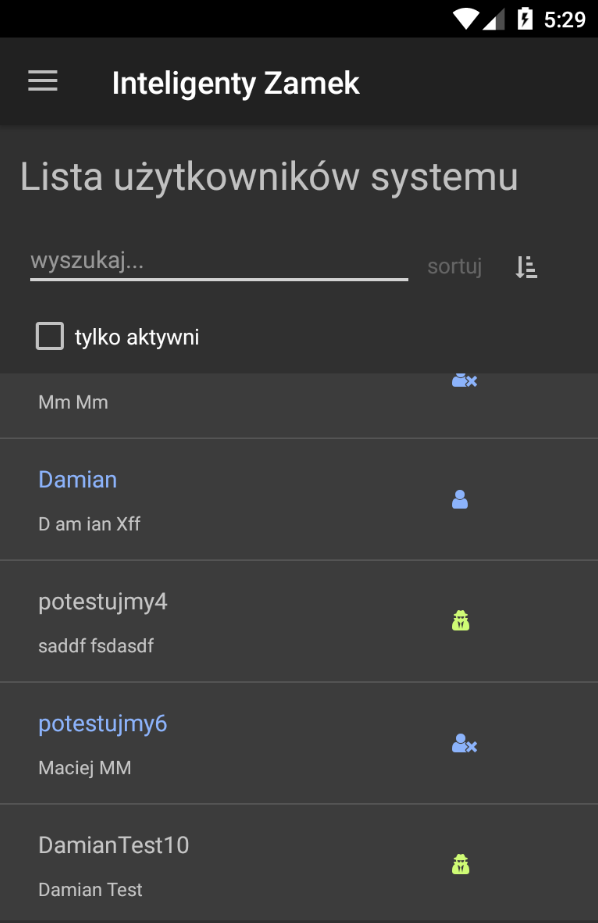
\includegraphics[width=12.5cm,height=8cm,keepaspectratio]
			{Obrazy/zarzadzanie_kontami}
			\caption{Panel zarządzania kontami użytkowników}
			\label{rys:rys:panel_Zarządzania_Kontami}
		
	\end{figure}
	
	\section*{Panel ustawień konta}
	W panelu ustawień użytkownik może zmienić hasło do swojego konta. Wymagane jest podanie starego hasła, a następnie nowego.Ponadto w panelu tym mamy podgląD certyfikatu szyfrujaćego wraz z możliwośćią wygenerowania nowego oraz zmiane adresu ip serwera  (Rysunek \ref{rys:panel_ustawienia_pionowo} i \ref{rys:panel_ustawienia_poziomo})
	
	\begin{figure}[ht!]
			\centering
			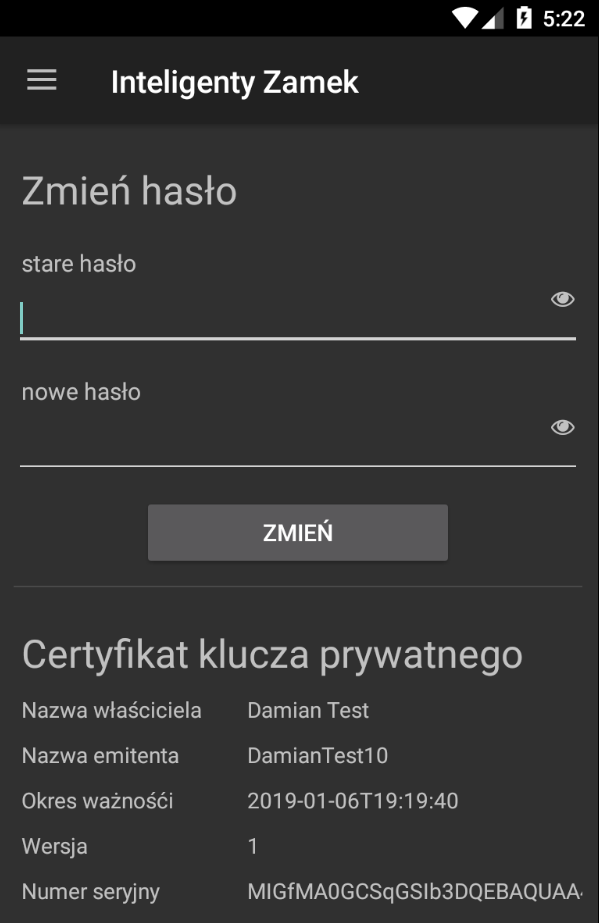
\includegraphics[width=12.5cm,height=8cm,keepaspectratio]
			{Obrazy/ustawienia_1}
			\caption{Panel ustawień konta (zmiana hasła)}
			\label{rys:panel_ustawienia_pionowo}
	\end{figure}
	\begin{figure}[ht!]
			\centering
		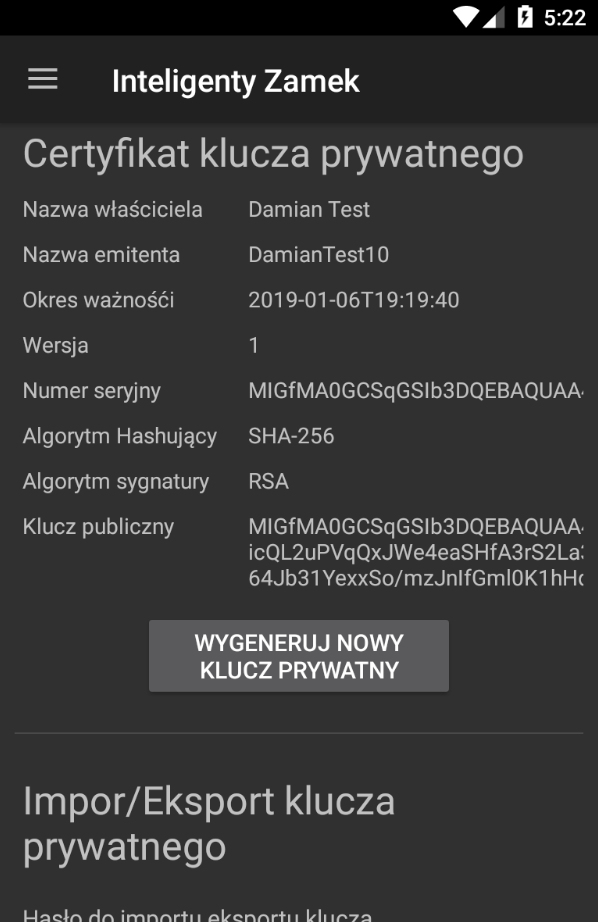
\includegraphics[width=12.5cm,height=8cm,keepaspectratio]
	{Obrazy/ustawienia_2}
	\caption{Panel ustawień konta (certyfikat szyfrująćy)}
	\label{rys:panel_ustawienia_pionowo}
\end{figure}
	\begin{figure}[ht!]
			\centering
		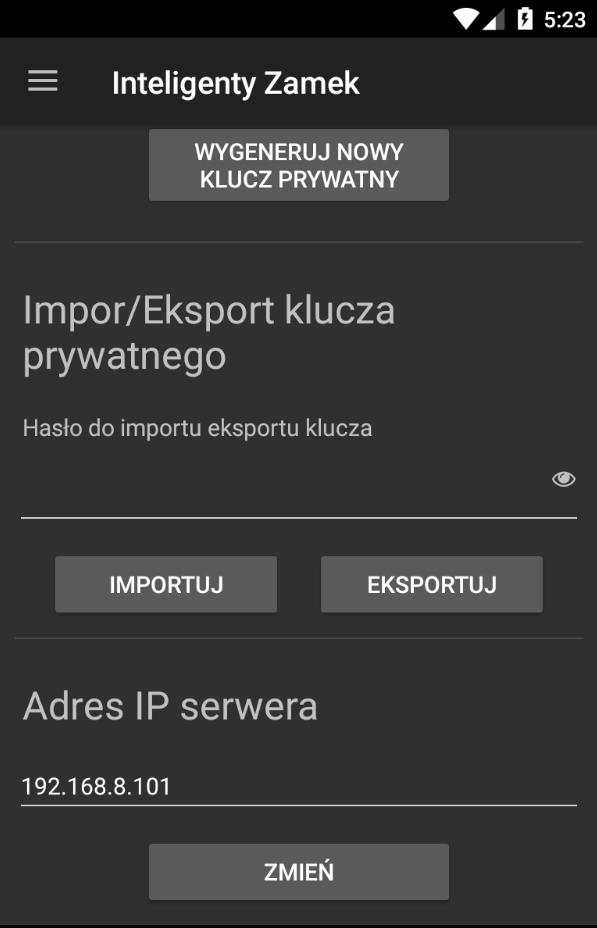
\includegraphics[width=12.5cm,height=8cm,keepaspectratio]
	{Obrazy/ustawienia_3}
	\caption{Panel ustawień konta (adres ip)}
	\label{rys:panel_ustawienia_pionowo}
\end{figure}
	\newpage
	
	
	
	
	\subsubsection{Widoki strony internetowej systemu}
	Strona internetowa posiada dwa widoki. Jeden jest to widok logowania  (Rysunek \ref{rys:strona_1} w któym administrator musi wpisać login oraz hasło. W drguim widoku mamy listę histori otwarcia zamków  (Rysunek \ref{rys:strona_2}) wraz z zaznaczeniem kolorystycznym która pokazuje czy była to próba autoryzowana.
	

\begin{figure}[ht!]
		\centering
	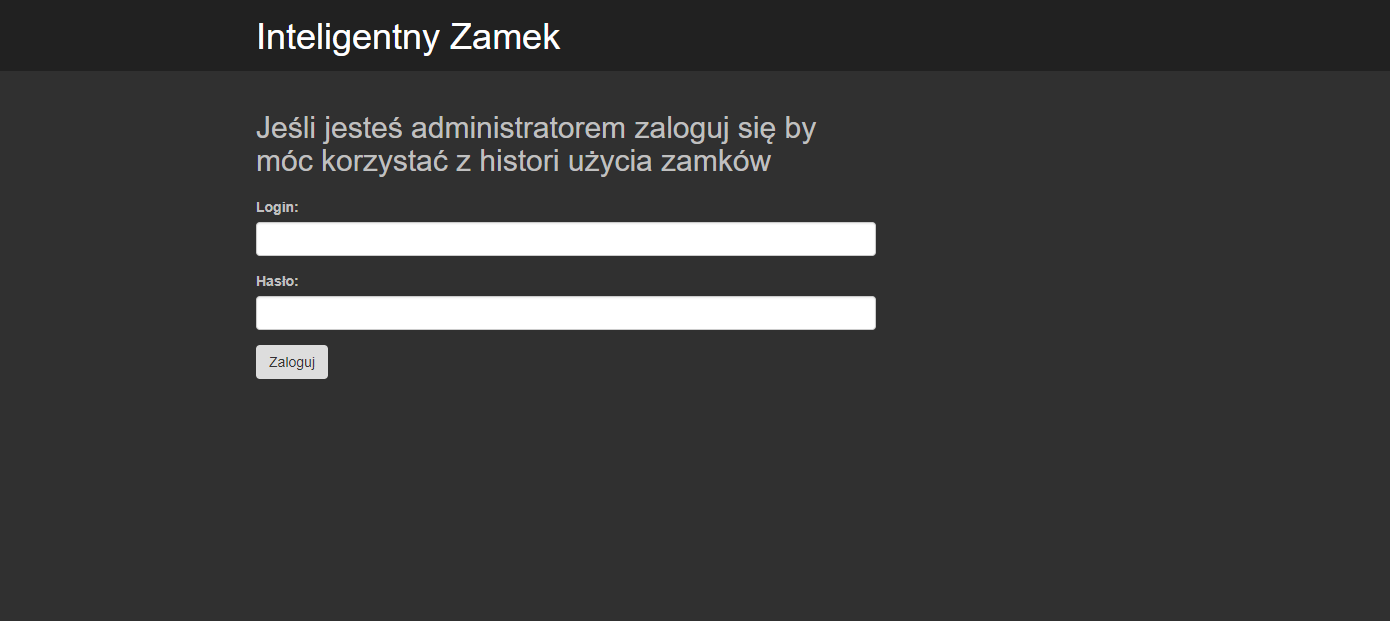
\includegraphics[width=12.5cm,height=10cm,keepaspectratio]
{Obrazy/strona_logowanie}
\caption{Strona logowania}
\label{rys:strona_1}
\end{figure}


\begin{figure}[ht!]
		\centering
	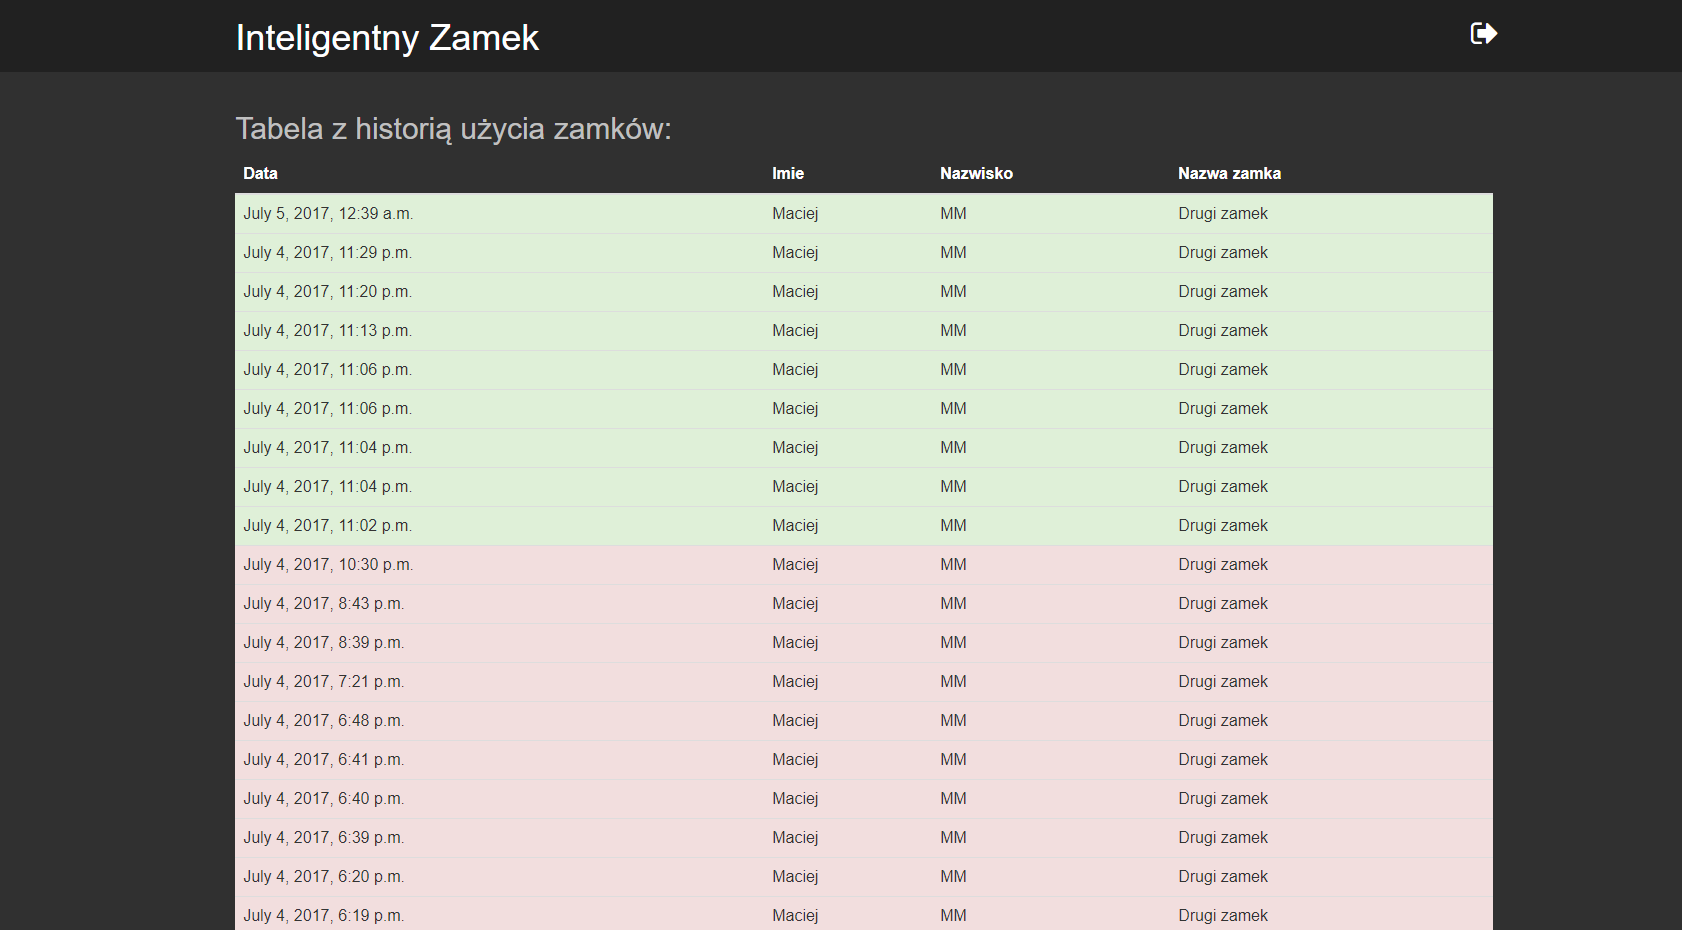
\includegraphics[width=12.5cm,height=10cm,keepaspectratio]
{Obrazy/strona_historia}
\caption{Strona z wyświetloną historią użycia zamkóW)}
\label{rys:strona_2}
\end{figure}
	
	\subsubsection{Komunikacja człowiek-interfejs}
	
		\paragraph{Komunikaty tekstowe}
		\paragraph{Symbolika ikon}
		\paragraph{Znaczenie kolorystyki}
		
	\subsubsection{Kolorystyka systemu}
	
\newpage
\subsection{Bezpieczeństwo systemu}
	\subsubsection{Projekt infrastruktury klucza publicznego (PKI)}
		\paragraph{Idea PKI}
		\paragraph{Urzedy certyfikujące}
		\paragraph{Klient systemu}
	\subsubsection{Poufność}
	\subsubsection{Dostępność}
	\subsubsection{Integralność}